\documentclass[11pt,a4paper,oneside]{book}
\usepackage[a4paper, portrait, margin=1.1in]{geometry}
% \documentclass[11pt,a4paper,twoside,openright]{book}
\usepackage{url}
\usepackage{makeidx}
\usepackage{listings}
\usepackage{graphicx}
\usepackage{fancyhdr}
\usepackage{fancyvrb}
\usepackage[usenames,dvipsnames]{color}


\definecolor{lightgray}{rgb}{.95,.95,.95}
\definecolor{darkgray}{rgb}{.4,.4,.4}
\definecolor{green}{rgb}{.2,.6,.0}
\definecolor{lightblue}{rgb}{.0,.5,.7}
\definecolor{purple}{rgb}{0.6, .1, 0.62}

\lstdefinelanguage{JavaScript}{
  keywords={typeof, new, true, false, catch, function, return, null, catch, switch, var, if, in, while, do, else, case, break, throw},
  keywordstyle=\color{blue}\bfseries,
  ndkeywords={exports, this},
  ndkeywordstyle=\color{lightblue}\bfseries,
  identifierstyle=\color{black},
  sensitive=false,
  comment=[l]{//},
  morecomment=[s]{/*}{*/},
  commentstyle=\color{green}\ttfamily,
  stringstyle=\color{purple}\ttfamily,
  morestring=[b]',
  morestring=[b]"
}

\lstdefinelanguage{KRE}{
  keywords={select, when, setting, with, http},
  keywordstyle=\color{blue}\bfseries,
  ndkeywords={rule},
  ndkeywordstyle=\color{lightblue}\bfseries,
  identifierstyle=\color{black},
  sensitive=false,
  morecomment=[s]{re\#}{\#},
  commentstyle=\color{green}\ttfamily,
  stringstyle=\color{purple}\ttfamily,
  morestring=[b]',
  morestring=[b]"
}

% \lstdefinelanguage{JSON}{
%   identifierstyle=\color{black},
%   sensitive=false,
%   stringstyle=\color{purple}\ttfamily,
%   morestring=[b]',
%   morestring=[b]"
% }

% \definecolor{numb}{RGB}{150, 150, 150}
% \definecolor{delim}{RGB}{20,105,176}

% \lstdefinelanguage{JSON}{
%   identifierstyle=\color{black},
%   sensitive=false,
%   stringstyle=\color{purple}\ttfamily,
%   morestring=[b]',
%   morestring=[b]",
%     literate=
%      *{0}{{{\color{numb}0}}}{1}
%       {1}{{{\color{numb}1}}}{1}
%       {2}{{{\color{numb}2}}}{1}
%       {3}{{{\color{numb}3}}}{1}
%       {4}{{{\color{numb}4}}}{1}
%       {5}{{{\color{numb}5}}}{1}
%       {6}{{{\color{numb}6}}}{1}
%       {7}{{{\color{numb}7}}}{1}
%       {8}{{{\color{numb}8}}}{1}
%       {9}{{{\color{numb}9}}}{1}
%       % {\{}{{{\color{delim}{\{}}}}{1}
%       % {\}}{{{\color{delim}{\}}}}}{1}
%       % {[}{{{\color{delim}{[}}}}{1}
%       % {]}{{{\color{delim}{]}}}}{1}
% }

\lstdefinelanguage{RDF}{
  keywords={on, insert, if, do, delete, let, in},
  keywordstyle=\color{blue}\bfseries,
  % keywords=[2]{delta},
  % keywordstyle=[2]\color{green}\bfseries,
  ndkeywords={document, resource},
  ndkeywordstyle=\color{lightblue}\bfseries,
  identifierstyle=\color{black},
  sensitive=false,
  comment=[l]{//},
  morecomment=[s]{/*}{*/},
  commentstyle=\color{green}\ttfamily,
  stringstyle=\color{purple}\ttfamily,
  morestring=[b]',
  morestring=[b]"
}

\lstdefinelanguage{N3}{
  alsoletter=?,
  keywords={ ?x },
  keywordstyle=\color{blue}\bfseries,
  ndkeywords={exports, this},
  ndkeywordstyle=\color{lightblue}\bfseries,
  identifierstyle=\color{black},
  sensitive=false,
  comment=[l]{//},
  morecomment=[s]{/*}{*/},
  commentstyle=\color{green}\ttfamily,
  stringstyle=\color{purple}\ttfamily,
  morestring=[b]',
  morestring=[b]"
}

\lstdefinelanguage{XChange}{
  keywords={TRANSACTION, on, end, in, insert, from},
  keywordstyle=\color{blue}\bfseries,
  ndkeywords={xchange, var, resource},
  ndkeywordstyle=\color{lightblue}\bfseries,
  identifierstyle=\color{black},
  sensitive=false,
  comment=[l]{//},
  morecomment=[s]{/*}{*/},
  commentstyle=\color{green}\ttfamily,
  stringstyle=\color{purple}\ttfamily,
  morestring=[b]',
  morestring=[b]"
}

\lstset{
  language=JavaScript,
  % backgroundcolor=\color{lightgray},
  extendedchars=true,
  basicstyle=\footnotesize\ttfamily,
  showstringspaces=false,
  showspaces=false,
  numbers=left,
  numberstyle=\tiny,
  numbersep=9pt,
  tabsize=2,
  breaklines=true,
  showtabs=false,
  captionpos=b,
  aboveskip=10pt,
  belowskip=10pt,
  xleftmargin=.3in,
  % frameround=tttt,
  boxpos=t
}


\makeatletter
\def\PY@reset{\let\PY@it=\relax \let\PY@bf=\relax%
    \let\PY@ul=\relax \let\PY@tc=\relax%
    \let\PY@bc=\relax \let\PY@ff=\relax}
\def\PY@tok#1{\csname PY@tok@#1\endcsname}
\def\PY@toks#1+{\ifx\relax#1\empty\else%
    \PY@tok{#1}\expandafter\PY@toks\fi}
\def\PY@do#1{\PY@bc{\PY@tc{\PY@ul{%
    \PY@it{\PY@bf{\PY@ff{#1}}}}}}}
\def\PY#1#2{\PY@reset\PY@toks#1+\relax+\PY@do{#2}}

\expandafter\def\csname PY@tok@gd\endcsname{\def\PY@tc##1{\textcolor[rgb]{0.63,0.00,0.00}{##1}}}
\expandafter\def\csname PY@tok@gu\endcsname{\let\PY@bf=\textbf\def\PY@tc##1{\textcolor[rgb]{0.50,0.00,0.50}{##1}}}
\expandafter\def\csname PY@tok@gt\endcsname{\def\PY@tc##1{\textcolor[rgb]{0.00,0.27,0.87}{##1}}}
\expandafter\def\csname PY@tok@gs\endcsname{\let\PY@bf=\textbf}
\expandafter\def\csname PY@tok@gr\endcsname{\def\PY@tc##1{\textcolor[rgb]{1.00,0.00,0.00}{##1}}}
\expandafter\def\csname PY@tok@cm\endcsname{\let\PY@it=\textit\def\PY@tc##1{\textcolor[rgb]{0.25,0.50,0.50}{##1}}}
\expandafter\def\csname PY@tok@vg\endcsname{\def\PY@tc##1{\textcolor[rgb]{0.10,0.09,0.49}{##1}}}
\expandafter\def\csname PY@tok@m\endcsname{\def\PY@tc##1{\textcolor[rgb]{0.40,0.40,0.40}{##1}}}
\expandafter\def\csname PY@tok@mh\endcsname{\def\PY@tc##1{\textcolor[rgb]{0.40,0.40,0.40}{##1}}}
\expandafter\def\csname PY@tok@go\endcsname{\def\PY@tc##1{\textcolor[rgb]{0.53,0.53,0.53}{##1}}}
\expandafter\def\csname PY@tok@ge\endcsname{\let\PY@it=\textit}
\expandafter\def\csname PY@tok@vc\endcsname{\def\PY@tc##1{\textcolor[rgb]{0.10,0.09,0.49}{##1}}}
\expandafter\def\csname PY@tok@il\endcsname{\def\PY@tc##1{\textcolor[rgb]{0.40,0.40,0.40}{##1}}}
\expandafter\def\csname PY@tok@cs\endcsname{\let\PY@it=\textit\def\PY@tc##1{\textcolor[rgb]{0.25,0.50,0.50}{##1}}}
\expandafter\def\csname PY@tok@cp\endcsname{\def\PY@tc##1{\textcolor[rgb]{0.74,0.48,0.00}{##1}}}
\expandafter\def\csname PY@tok@gi\endcsname{\def\PY@tc##1{\textcolor[rgb]{0.00,0.63,0.00}{##1}}}
\expandafter\def\csname PY@tok@gh\endcsname{\let\PY@bf=\textbf\def\PY@tc##1{\textcolor[rgb]{0.00,0.00,0.50}{##1}}}
\expandafter\def\csname PY@tok@ni\endcsname{\let\PY@bf=\textbf\def\PY@tc##1{\textcolor[rgb]{0.60,0.60,0.60}{##1}}}
\expandafter\def\csname PY@tok@nl\endcsname{\def\PY@tc##1{\textcolor[rgb]{0.63,0.63,0.00}{##1}}}
\expandafter\def\csname PY@tok@nn\endcsname{\let\PY@bf=\textbf\def\PY@tc##1{\textcolor[rgb]{0.00,0.00,1.00}{##1}}}
\expandafter\def\csname PY@tok@no\endcsname{\def\PY@tc##1{\textcolor[rgb]{0.53,0.00,0.00}{##1}}}
\expandafter\def\csname PY@tok@na\endcsname{\def\PY@tc##1{\textcolor[rgb]{0.49,0.56,0.16}{##1}}}
\expandafter\def\csname PY@tok@nb\endcsname{\def\PY@tc##1{\textcolor[rgb]{0.00,0.50,0.00}{##1}}}
\expandafter\def\csname PY@tok@nc\endcsname{\let\PY@bf=\textbf\def\PY@tc##1{\textcolor[rgb]{0.00,0.00,1.00}{##1}}}
\expandafter\def\csname PY@tok@nd\endcsname{\def\PY@tc##1{\textcolor[rgb]{0.67,0.13,1.00}{##1}}}
\expandafter\def\csname PY@tok@ne\endcsname{\let\PY@bf=\textbf\def\PY@tc##1{\textcolor[rgb]{0.82,0.25,0.23}{##1}}}
\expandafter\def\csname PY@tok@nf\endcsname{\def\PY@tc##1{\textcolor[rgb]{0.00,0.00,1.00}{##1}}}
\expandafter\def\csname PY@tok@si\endcsname{\let\PY@bf=\textbf\def\PY@tc##1{\textcolor[rgb]{0.73,0.40,0.53}{##1}}}
\expandafter\def\csname PY@tok@s2\endcsname{\def\PY@tc##1{\textcolor[rgb]{0.73,0.13,0.13}{##1}}}
\expandafter\def\csname PY@tok@vi\endcsname{\def\PY@tc##1{\textcolor[rgb]{0.10,0.09,0.49}{##1}}}
\expandafter\def\csname PY@tok@nt\endcsname{\let\PY@bf=\textbf\def\PY@tc##1{\textcolor[rgb]{0.00,0.50,0.00}{##1}}}
\expandafter\def\csname PY@tok@nv\endcsname{\def\PY@tc##1{\textcolor[rgb]{0.10,0.09,0.49}{##1}}}
\expandafter\def\csname PY@tok@s1\endcsname{\def\PY@tc##1{\textcolor[rgb]{0.73,0.13,0.13}{##1}}}
\expandafter\def\csname PY@tok@sh\endcsname{\def\PY@tc##1{\textcolor[rgb]{0.73,0.13,0.13}{##1}}}
\expandafter\def\csname PY@tok@sc\endcsname{\def\PY@tc##1{\textcolor[rgb]{0.73,0.13,0.13}{##1}}}
\expandafter\def\csname PY@tok@sx\endcsname{\def\PY@tc##1{\textcolor[rgb]{0.00,0.50,0.00}{##1}}}
\expandafter\def\csname PY@tok@bp\endcsname{\def\PY@tc##1{\textcolor[rgb]{0.00,0.50,0.00}{##1}}}
\expandafter\def\csname PY@tok@c1\endcsname{\let\PY@it=\textit\def\PY@tc##1{\textcolor[rgb]{0.25,0.50,0.50}{##1}}}
\expandafter\def\csname PY@tok@kc\endcsname{\let\PY@bf=\textbf\def\PY@tc##1{\textcolor[rgb]{0.00,0.50,0.00}{##1}}}
\expandafter\def\csname PY@tok@c\endcsname{\let\PY@it=\textit\def\PY@tc##1{\textcolor[rgb]{0.25,0.50,0.50}{##1}}}
\expandafter\def\csname PY@tok@mf\endcsname{\def\PY@tc##1{\textcolor[rgb]{0.40,0.40,0.40}{##1}}}
%\expandafter\def\csname PY@tok@err\endcsname{\def\PY@bc##1{\setlength{\fboxsep}{0pt}\fcolorbox[rgb]{1.00,0.00,0.00}{1,1,1}{\strut ##1}}}
\expandafter\def\csname PY@tok@kd\endcsname{\let\PY@bf=\textbf\def\PY@tc##1{\textcolor[rgb]{0.00,0.50,0.00}{##1}}}
\expandafter\def\csname PY@tok@ss\endcsname{\def\PY@tc##1{\textcolor[rgb]{0.10,0.09,0.49}{##1}}}
\expandafter\def\csname PY@tok@sr\endcsname{\def\PY@tc##1{\textcolor[rgb]{0.73,0.40,0.53}{##1}}}
\expandafter\def\csname PY@tok@mo\endcsname{\def\PY@tc##1{\textcolor[rgb]{0.40,0.40,0.40}{##1}}}
\expandafter\def\csname PY@tok@kn\endcsname{\let\PY@bf=\textbf\def\PY@tc##1{\textcolor[rgb]{0.00,0.50,0.00}{##1}}}
\expandafter\def\csname PY@tok@mi\endcsname{\def\PY@tc##1{\textcolor[rgb]{0.40,0.40,0.40}{##1}}}
\expandafter\def\csname PY@tok@gp\endcsname{\let\PY@bf=\textbf\def\PY@tc##1{\textcolor[rgb]{0.00,0.00,0.50}{##1}}}
\expandafter\def\csname PY@tok@o\endcsname{\def\PY@tc##1{\textcolor[rgb]{0.40,0.40,0.40}{##1}}}
\expandafter\def\csname PY@tok@kr\endcsname{\let\PY@bf=\textbf\def\PY@tc##1{\textcolor[rgb]{0.00,0.50,0.00}{##1}}}
\expandafter\def\csname PY@tok@s\endcsname{\def\PY@tc##1{\textcolor[rgb]{0.73,0.13,0.13}{##1}}}
\expandafter\def\csname PY@tok@kp\endcsname{\def\PY@tc##1{\textcolor[rgb]{0.00,0.50,0.00}{##1}}}
\expandafter\def\csname PY@tok@w\endcsname{\def\PY@tc##1{\textcolor[rgb]{0.73,0.73,0.73}{##1}}}
\expandafter\def\csname PY@tok@kt\endcsname{\def\PY@tc##1{\textcolor[rgb]{0.69,0.00,0.25}{##1}}}
\expandafter\def\csname PY@tok@ow\endcsname{\let\PY@bf=\textbf\def\PY@tc##1{\textcolor[rgb]{0.67,0.13,1.00}{##1}}}
\expandafter\def\csname PY@tok@sb\endcsname{\def\PY@tc##1{\textcolor[rgb]{0.73,0.13,0.13}{##1}}}
\expandafter\def\csname PY@tok@k\endcsname{\let\PY@bf=\textbf\def\PY@tc##1{\textcolor[rgb]{0.00,0.50,0.00}{##1}}}
\expandafter\def\csname PY@tok@se\endcsname{\let\PY@bf=\textbf\def\PY@tc##1{\textcolor[rgb]{0.73,0.40,0.13}{##1}}}
\expandafter\def\csname PY@tok@sd\endcsname{\let\PY@it=\textit\def\PY@tc##1{\textcolor[rgb]{0.73,0.13,0.13}{##1}}}
%\expandafter\def\csname PY@tok@err\endcsname{}

\def\PYZbs{\char`\\}
\def\PYZus{\char`\_}
\def\PYZob{\char`\{}
\def\PYZcb{\char`\}}
\def\PYZca{\char`\^}
\def\PYZam{\char`\&}
\def\PYZlt{\char`\<}
\def\PYZgt{\char`\>}
\def\PYZsh{\char`\#}
\def\PYZpc{\char`\%}
\def\PYZdl{\char`\$}
\def\PYZhy{\char`\-}
\def\PYZsq{\char`\'}
\def\PYZdq{\char`\"}
\def\PYZti{\char`\~}
% for compatibility with earlier versions
\def\PYZat{@}
\def\PYZlb{[}
\def\PYZrb{]}
\makeatother

% How deep numbering is applied to titles
\setcounter{secnumdepth}{3}
% \setcounter{tocdepth}{3}

% Prepare the word index
\makeindex

% Prepare header and footer
\pagestyle{fancy}
\fancyhf{}
\rhead{\footnotesize\leftmark}
\lfoot{Towards the Reactive Web}
\rfoot{\thepage}
\renewcommand{\headrulewidth}{0.3pt}
\renewcommand{\footrulewidth}{0.3pt}

% Apply page style also to chapter's first page
\makeatletter
\renewcommand\chapter{\if@openright\cleardoublepage\else\clearpage\fi
  \thispagestyle{fancy}%
  \global\@topnum\z@
  \@afterindentfalse
  \secdef\@chapter\@schapter}
\makeatother


\begin{document}

\frontmatter
	\begin{titlepage}
\begin{center}

% \title{\huge \textbf{Towards The Reactive Web}\vspace*{15 mm}}
% %\subtitle{Master Thesis Report}
% \date{\today}
% %\date{}
% %\author{Dominic Bosch \\ Departement Mathematics and Computer Science \\ University of Basel}
% \author{\fontsize{11}{9}\selectfont
% Master Thesis\\
% \vspace*{10 mm}\\
% Dominic Bosch\\
% Departement Mathematics and Computer Science\\
% University of Basel
% }
% \maketitle

\vspace*{4cm}
\HRule \\[0.4cm]
{ \huge \bfseries Towards Reactive Information Systems \\ and their Services \\[0.4cm] }
% { \huge \bfseries Towards The Reactive Web \\[0.4cm] }
\HRule \\[1.5cm]

% \textsc{\Large Departement Mathematics and Computer Science}\\[0.5cm]

\vspace*{.5cm}
\textit{\textsc{\LARGE Master Thesis}}\\
\vspace*{2.5cm}

% Author and supervisor
\begin{minipage}{0.4\textwidth}
\begin{flushleft} \large
\emph{Author:}\\
Dominic \textsc{Bosch}
\end{flushleft}
\end{minipage}
\begin{minipage}{0.4\textwidth}
\begin{flushright} \large
\emph{Supervisors:} \\
Prof. Dr.~Helmar \textsc{Burkhart}\\
Dr.~Martin \textsc{Guggisberg}
\end{flushright}
\end{minipage}

\vfill

% Bottom of the page
{\large May 15, 2014} \\[1.5cm]



% \textsc{\LARGE University of Basel}\\

\includegraphics[width=0.15\textwidth]{figures/unilogoschwarz}~\\[1cm]
\end{center}
\end{titlepage}

	\chapter*{Acknowledgment}
I would like to express my deep gratitude to my master thesis advisor, Prof. Dr. Helmar Burkhart, for his patience and constant encouragement to keep going further.
I also want to thank Dr. Martin Guggisberg for his very helpful advices and hints to existing technologies.
Besides my advisors, I would like to thank the members of the research group: Danilo Guerrera,
Antonio Maffia, Alexander Gr\"oflin and Robert Frank for their help, many interesting discussions and inputs.

I would like to thank my parents Silvia and Peter Bosch for their love, patience and financial support on my journey.
Special thanks go to my sister Svenja, her husband Andreas and their seven months old son Nico, who all kept me going with their joyfulness and irresistble smiling.
Finally I would like to thank my partner Kathrina Hagnauer for her patience and endless love.
	\tableofcontents

\mainmatter
	\chapter{Introduction}

The fast evolving web has brought up a trend towards easy to master interfaces to services, the so called WebAPIs.
\index{WebAPI}
They do not only provide access to mere services but whole applications that allow access over WebAPIs.
These trending WebAPIs benefit from a RESTful architecture which predominantly uses HTTP and thus relies on the most basic and powerful operations and the basis of the Web itself, the HTTP protocol. 


% TODO Enough on WebAPI's?

% quick (handling/mastering) accessible services and even whole web applications through so called Web APIs.
% WebAPIs provide powerful tools to govern data and functionality in the web independently of any user interface from the service provider.
% The relatively
% Allowing access to these services via API is increasingly popular and allows to mash up these services

% Practically all services flood the user with events
% The web should be event driven, that's why we need an engine that deals with events and makes the web reactive
% There's still the challenge of filtering
% What's important to whom
% Plus the user needs to have tools to combine and add programmability to the combination,( such as conditions, selection of provided arguments and so on)

% % TODO Reactivity
% \index{Reactivity}

% % TODO Programmability of the Web
% \index{Programmability}

% % TODO Event Trigger
% \index{Event}
% \index{Event Trigger}

% % TODO Actions
% \index{Actions}

% % TODO engine
% \index{Engine}

% % TODO Webhooks
% \index{Webhooks}


\section{WebAPI Mashups}
\index{WebAPI Mashups}
Mashups combine information and functionality of more than one resource in a single place.
The mashing up of such resources allows new points of view on data, or even ways to interact with them.
Simple functions are combined into more powerful ones which influence data and services in a way their founders eventually didn't even think of.
They have been developped ever since services in the web started to exist and were accessible in a more or less convenient way.
One of the earliest inventors of such a webservice mashup is Paul Rademacher.
In the same year after Google Maps came up in 2005, he invented a site\cite{wwwRademacherOne,wwwRademacherTwo} that displayed Craigslist houses on a Google Map.
With no Google Maps API at that time, he needed time and skills to reverse engineer Google Map's functionalities.


A large number of such "static" mashups were and are still developped.
They are static in the way that they aggregate a fixed (and mostly low) number, of either data or functionality resources, to provide an enhanced resource in a specialized domain.
Of course Mashups can be mashed up again, to provide even more sophisticated functionality and data.
Some latest example Mashups, taken from the ProgrammableWeb\cite{wwwProgrammableWeb} directory, are:

\begin{itemize}
  \item Wifi and Plugs\cite{wwwWifiAndPlugs}: MapBox, Google Docs and Import.io API's used to display where Wi-Fi and plugs are available in London.
  \item MapLight\cite{wwwMapLight}: GovTrack.us and OpenSecrets API's used to combine political results with financial contributions to show how capital contributions affect voting.
  \item Shared Count\cite{wwwSharedCount}: Facebook, LinkedIn, Pinterest and Twitter API's used to display informations about how well spread a URL is on social media sites.
\end{itemize}

In the past few years, research and development for platforms to allow users to flexibly mashup WebAPIs got attention.
With IFTTT and Zapier, two platforms have evolved out of this process.
Users that register on those platforms are provided with a multitude of WebAPI functions that act as event triggers and such that are used to execute actions.
The user is then free to combine these event triggers and actions in the way it suits best, creating helpful WebAPI mashups on their own.

% Since this is a quite new field the why and how is hidden from the research.
% you need events
% you need rules / rule language





\section{Rule Languages}
\index{Rules}
\index{Rule Language}

% TODO
% To allow user-defined WebAPI mashups, a rule language is required which is capable to express ECA Rules. 


% TODO
% ECA
% \index{ECA}

%TODO Table with categorization of Rule languages

Several different rule languages have been developped for different purposes over the last years and they vary grately in their purpose.
% terms of usability for ECA Rules together with WebAPI mashups.
A compilation of research on different emerging rule-based languages and technologies \cite{2009-Paschke_Boley-RCER.pdf} gives an oveview over such efforts.
We examined different existing rule languages with respect to a certain use case to identify its applicability for reactivity in the web. % TODO find other word as applicability
The use case is defined such that the rule needs to suffice the ECA paradigm:

\begin{itemize}
  \item Event: Receipt of an Email
  \item Condition: Check for a certain sender
  \item Action: Store it remotely via a WebAPI
\end{itemize}

We defined an email event which the rule languages need to be able to process.
The JSON representation of the given email event is shown in Listing~\ref{lstemail}.

\begin{Verbatim}[frame=single,fontsize=\footnotesize,commandchars=\\\{\},numbers=left,firstnumber=1,stepnumber=1,xleftmargin
=.3in]
\PY{p}{\PYZob{}}
  \PY{n+nt}{\PYZdq{}eventname\PYZdq{}}\PY{p}{:} \PY{l+s+s2}{\PYZdq{}email\PYZdq{}}\PY{p}{,}
  \PY{n+nt}{\PYZdq{}body\PYZdq{}}\PY{p}{:} \PY{p}{\PYZob{}}
    \PY{n+nt}{\PYZdq{}sender\PYZdq{}}\PY{p}{:} \PY{l+s+s2}{\PYZdq{}sender@mail.com\PYZdq{}}\PY{p}{,}
    \PY{n+nt}{\PYZdq{}subject\PYZdq{}}\PY{p}{:} \PY{l+s+s2}{\PYZdq{}Important subject!\PYZdq{}}\PY{p}{,}
    \PY{n+nt}{\PYZdq{}textbody\PYZdq{}}\PY{p}{:} \PY{l+s+s2}{\PYZdq{}Hi User,\PYZbs{}n\PYZbs{}nThis is a lengthy mail body\PYZdq{}}
  \PY{p}{\PYZcb{}}
\PY{p}{\PYZcb{}}
\end{Verbatim}
\begin{lstlisting}[label=lstemail,caption=Example E-Mail event expressed in JSON]
\end{lstlisting}

\subsection{RDF \& XML}
\index{RDF}
\index{XML}
An early ECA Rule Language for XML repositories\cite{Papamarkos03event-condition-actionrule} was postulated in 2003 and was picked up by many researches afterwards. It was designed to react on insert and delete events within XML repositories and as an action change XML documents.

\begin{lstlisting}[frame=single,float=h,label=lstrdf,language=RDF,caption=E-Mail Example rule expressed in RDF]
	ON INSERT document(’inbound_queue.xml’)/mails/mail
	IF $delta/sender[.=’sender@mail.com’]
	DO DELETE document(’inbound_queue.xml’)/mails/mail;
		LET $api = resource("www.webapi.com") IN
		INSERT ($api, newcontent,
			<content>New mail: {$delta/subject}</content>)
\end{lstlisting}


Now apart from implementing a rules engine, we would also need to add an XML document event manager which interpretes and pushes events into the XML file \emph{inbound\_queue.xml}. Then again this instance would interprete the ouptuts of the ECA engine, which would theoretically manifest in other XML documents, and produce meaningful actions on remote hosts. This wouldn't be an architecture which has its focus on the solution of our use case and, as a result, add complexity and create an unnecessary overhead.

\subsection{Notation 3}
\index{Notation 3}
To make the lengthy RDF definitions smaller and more readable, Notation 3\cite{wwwn3} was designed and announced in 2005. Through the implies operator(=\textgreater) an "event" can be connected to an "action", both expressed in RDF's subject, predicate, object notation, which makes the expression of ECA rules a complicated and not very intuitive task. A solution to our use case would look as follows:

\begin{lstlisting}[frame=single,float=h,label=lstn3,language=N3,caption=E-Mail Example rule expressed in Notation 3]
	{ ?x :event "email". ?x :sender "sender@mail.com" }
		=> { :webapi :newcontent ?x }
\end{lstlisting}


It's obvious that this language is used to express relations between entities and thus not really suitable for our use case, since we would require another interpreter to infer the actions. But concepts and ideas of the work that was done in these consortias could eventually still find influence into our solution.

\subsection{XChange/Xcerpt}
\index{XChange}\index{Xcerpt}
The rule language XChange\cite{2005-Patranjan-TLE.pdf} was the outcome of the REWERSE project and acted as an influence in many further researches. The language was designed to add reactive behaviour to a "static" web which is represented through XML resources. Thus we have action logics to alter such resources through insertions and deletions. Since we aim to utilize web API's for our rule language we need a more generic approach which adds flexibility in term of the API provided. But the thorough research done with the language XChange holds valuable concepts, especially in terms of temporal evet composition. This could be a rule according to our use case:

\begin{lstlisting}[frame=single,float=h,label=lstxchange1,language=XChange,caption=E-Mail Example rule expressed in XChange]
	TRANSACTION
		in {
			resource { "http://www.webapi.com"},
			newcontents {{
				insert newcontent { var Mail }
			}}
		}
	ON
		xchange:event {{
			xchange:sender { "http://mailserver.com" },
			var Mail -> email {{
				sender { "sender@mail.com" }
			}}
		}}
	END
\end{lstlisting}

But XChange is designed to access other resources in an action and thus provides powerful tools:

\begin{lstlisting}[frame=single,float=h,label=lstxchange2,language=XChange,caption=XChange Rule accesses remote resource]
	TRANSACTION
		[...]
	ON
		[...]
	FROM
		in {
			resource { "http://www.weather.com"},
			temperatures {{
				var T -> temperature {{
					datetime { "2013-10-20-08:00:00AM" }
				}}
			}}
		}
	END
\end{lstlisting}

\subsection{JSON Rules}
\index{JSON Rules}
In 2008 \emph{JSON Rules}~\cite{2008-Giurca_Pascalau-JSON_Rules.pdf} was introduced as a language to easily react on specific DOM tree compositions.
The usage of JavaScript allowed them to provide simple functions which could be called directly by the actions, thus abstracting functionality from the language.
This key concept found influence into our language as it allows different layers of abstractions.
Through this it is possible to provide generic functions for expert user as well as very limited functions with only few possibilities for parameterization to be used by unexperienced persons.
A drawback of this language is its binding to DOM tree events, where we would want to react on any events happening in the world.
Also the temporal composition to complex events is not a subject of their work and needs further attention.


\begin{Verbatim}[frame=single,fontsize=\footnotesize,commandchars=\\\{\},numbers=left,firstnumber=1,stepnumber=1,xleftmargin
=.3in]
\PY{p}{\PYZob{}}
    \PY{n+nt}{\PYZdq{}id\PYZdq{}}\PY{p}{:} \PY{l+m+mi}{0}\PY{p}{,}
    \PY{n+nt}{\PYZdq{}conditions\PYZdq{}}\PY{p}{:} \PY{p}{[}
        \PY{p}{\PYZob{}}
            \PY{n+nt}{\PYZdq{}type\PYZdq{}}\PY{p}{:} \PY{l+s+s2}{\PYZdq{}email\PYZdq{}}\PY{p}{,}
            \PY{n+nt}{\PYZdq{}constraints\PYZdq{}}\PY{p}{:} \PY{p}{[}
                \PY{p}{\PYZob{}}
                    \PY{n+nt}{\PYZdq{}propertyName\PYZdq{}}\PY{p}{:} \PY{l+s+s2}{\PYZdq{}sender\PYZdq{}}\PY{p}{,}
                    \PY{n+nt}{\PYZdq{}operator\PYZdq{}}\PY{p}{:} \PY{l+s+s2}{\PYZdq{}EQ\PYZdq{}}\PY{p}{,}
                    \PY{n+nt}{\PYZdq{}restriction\PYZdq{}}\PY{p}{:} \PY{p}{\PYZob{}}
                        \PY{n+nt}{\PYZdq{}type\PYZdq{}}\PY{p}{:} \PY{l+s+s2}{\PYZdq{}String\PYZdq{}}\PY{p}{,}
                        \PY{n+nt}{\PYZdq{}value\PYZdq{}}\PY{p}{:} \PY{l+s+s2}{\PYZdq{}sender@mail.com\PYZdq{}}
                    \PY{p}{\PYZcb{}}
                \PY{p}{\PYZcb{}}\PY{p}{,}
                \PY{p}{\PYZob{}}
                    \PY{n+nt}{\PYZdq{}bind\PYZdq{}}\PY{p}{:} \PY{l+s+s2}{\PYZdq{}\PYZdl{}S\PYZdq{}}\PY{p}{,}
                    \PY{n+nt}{\PYZdq{}propertyName\PYZdq{}}\PY{p}{:} \PY{l+s+s2}{\PYZdq{}subject\PYZdq{}}
                \PY{p}{\PYZcb{}}
            \PY{p}{]}
        \PY{p}{\PYZcb{}}
    \PY{p}{]}\PY{p}{,}
    \PY{n+nt}{\PYZdq{}actions\PYZdq{}}\PY{p}{:} \PY{p}{[}
        \PY{l+s+s2}{\PYZdq{}webapi(\PYZsq{}addcontent\PYZsq{}, \PYZdl{}S)\PYZdq{}}
    \PY{p}{]}
\PY{p}{\PYZcb{}}
\end{Verbatim}
\begin{lstlisting}[caption=E-Mail Example rule in JSON Rules]
\end{lstlisting}


\subsection{Kinetics Rule Language (KRL)}
\index{KRL}
A most recent (2011) open-source development is the Kinetic Rules Engine together with the Kinetics Rule Language~\cite{bookTheLiveWeb}.
It is built for the purpose of adding reactivity to the cloud.
The language is based on declarative syntax, enriched with imparative elements.
But it is a tedious task to get into a whole new language and their caveats.
\emph{authorization?}

\begin{lstlisting}[frame=single,float=h,label=lstkre,language=KRE,caption=E-Mail Example rule in KRL]
	rule store_mail {
		select when mail newmail
		sender re#sender@mail.com#
		subject re#*# setting(subj)
		http:post("http://www.webapi.com/newcontent")
		with params = {
			"text": subj
		}
	}
\end{lstlisting}


\subsection{(Reaction) RuleML}
\index{RuleML}
The basis of \emph{RuleML}~\cite{2006-Boley-RuleML.pdf} is datalog, a language in the intersection of SQL and Prolog.
In 2012 the \emph{Reaction RuleML}~\cite{2012-Paschke_etal-ReactionRuleML.pdf} language incorporated several different types of rules into the RuleML syntax, to establish a uniform syntax and interchangability of rules.
\emph{Reaction RuleML} is a valuable resource in terms of manifold research that has been done in the domain of rule languages, but the syntax is not user-friendly.


R2ML allows usage for RuleML together with many other dialects. Really!?

\begin{Verbatim}[frame=single,fontsize=\footnotesize,commandchars=\\\{\},numbers=left,firstnumber=1,stepnumber=1,xleftmargin
=.3in]
  \PY{n+nt}{\PYZlt{}Rule} \PY{n+na}{style=}\PY{l+s}{\PYZdq{}active\PYZdq{}}\PY{n+nt}{\PYZgt{}}
    \PY{n+nt}{\PYZlt{}on}\PY{n+nt}{\PYZgt{}}
      \PY{n+nt}{\PYZlt{}Event}\PY{n+nt}{\PYZgt{}}
        \PY{n+nt}{\PYZlt{}Atom}\PY{n+nt}{\PYZgt{}}
          \PY{n+nt}{\PYZlt{}Rel} \PY{n+na}{per=}\PY{l+s}{\PYZdq{}value\PYZdq{}}\PY{n+nt}{\PYZgt{}}mail\PY{n+nt}{\PYZlt{}/Rel\PYZgt{}}
          \PY{n+nt}{\PYZlt{}Var}\PY{n+nt}{\PYZgt{}}sender\PY{n+nt}{\PYZlt{}/Var\PYZgt{}}
          \PY{n+nt}{\PYZlt{}Var}\PY{n+nt}{\PYZgt{}}subject\PY{n+nt}{\PYZlt{}/Var\PYZgt{}}
        \PY{n+nt}{\PYZlt{}/Atom\PYZgt{}}
      \PY{n+nt}{\PYZlt{}/Event\PYZgt{}}
    \PY{n+nt}{\PYZlt{}/on\PYZgt{}}
    \PY{n+nt}{\PYZlt{}if}\PY{n+nt}{\PYZgt{}}
      \PY{n+nt}{\PYZlt{}Atom}\PY{n+nt}{\PYZgt{}}
        \PY{n+nt}{\PYZlt{}op}\PY{n+nt}{\PYZgt{}}\PY{n+nt}{\PYZlt{}Rel}\PY{n+nt}{\PYZgt{}}equals\PY{n+nt}{\PYZlt{}/Rel\PYZgt{}}\PY{n+nt}{\PYZlt{}/op\PYZgt{}}
        \PY{n+nt}{\PYZlt{}Var}\PY{n+nt}{\PYZgt{}}sender\PY{n+nt}{\PYZlt{}/Var\PYZgt{}}
        \PY{n+nt}{\PYZlt{}Ind}\PY{n+nt}{\PYZgt{}}sender@mail.com\PY{n+nt}{\PYZlt{}/Ind\PYZgt{}}
      \PY{n+nt}{\PYZlt{}/Atom\PYZgt{}}
    \PY{n+nt}{\PYZlt{}/if\PYZgt{}}
    \PY{n+nt}{\PYZlt{}do}\PY{n+nt}{\PYZgt{}}
      \PY{n+nt}{\PYZlt{}Atom}\PY{n+nt}{\PYZgt{}}
        \PY{n+nt}{\PYZlt{}oid}\PY{n+nt}{\PYZgt{}}\PY{n+nt}{\PYZlt{}Ind} \PY{n+na}{uri=}\PY{l+s}{\PYZdq{}http://webapi.com\PYZdq{}}\PY{n+nt}{/\PYZgt{}}\PY{n+nt}{\PYZlt{}/oid\PYZgt{}}
        \PY{n+nt}{\PYZlt{}Rel}\PY{n+nt}{\PYZgt{}}newcontent\PY{n+nt}{\PYZlt{}/Rel\PYZgt{}}
        \PY{n+nt}{\PYZlt{}Var}\PY{n+nt}{\PYZgt{}}subject\PY{n+nt}{\PYZlt{}/Var\PYZgt{}} 
      \PY{n+nt}{\PYZlt{}/Atom\PYZgt{}}
    \PY{n+nt}{\PYZlt{}/do\PYZgt{}}
  \PY{n+nt}{\PYZlt{}/Rule\PYZgt{}}
\end{Verbatim}


%\section{Conclusion}
Most of the examined rule languages are designed for the interchangability of rules between different service providers. We do not attempt to jump into this domain but we rather pick up important concepts to manifest web API's as first class citizens of our rule language. This allows the ad-hoc design and implementation of reactive rules between existing web API's without the need for their cooperation in setting up their endpoint in a special way.
	
\chapter{Conceptual Model for Reactive Web Systems}
% NOTES / TODOs:
%
% Rahmenbedingungen
% Vorzuege
% Notwendigkeiten
% Architektur


% NOTES / TODOs:
%
% Model / Schema
% Zeit / Verteiltheit
% RL <-> ECA
% why are we now suddenly responsive? we loosened up certain things



% \section{Event Condition Action (ECA) Model in the Web}
In the last section we showed how mashups create additional value for the web by combining several WebAPI's.
But it turned out, that such mashups are closed systems, which ofen only allow little degree of parametrization.
To get past such limitations and define a conceptual model for reactive web systems, it is necessary to define a 

existing rule languages, rule engines, 

Existing ECA systems all act on local data.
% (List examples) 
Looking at (Wikipedia...) their definition is actions on local data.
This does only add reactivity to these systems and not to the Web per se.

Such systems are merely event sinks which add fairly any value to the Web, except for the individual users and the system itself.
We are taking a step further and allow not only the chaining up of several remote ECA engines, but also the invocation of actions on any arbitrary Web accessible service.

\begin{figure}[h!]
  \centering
  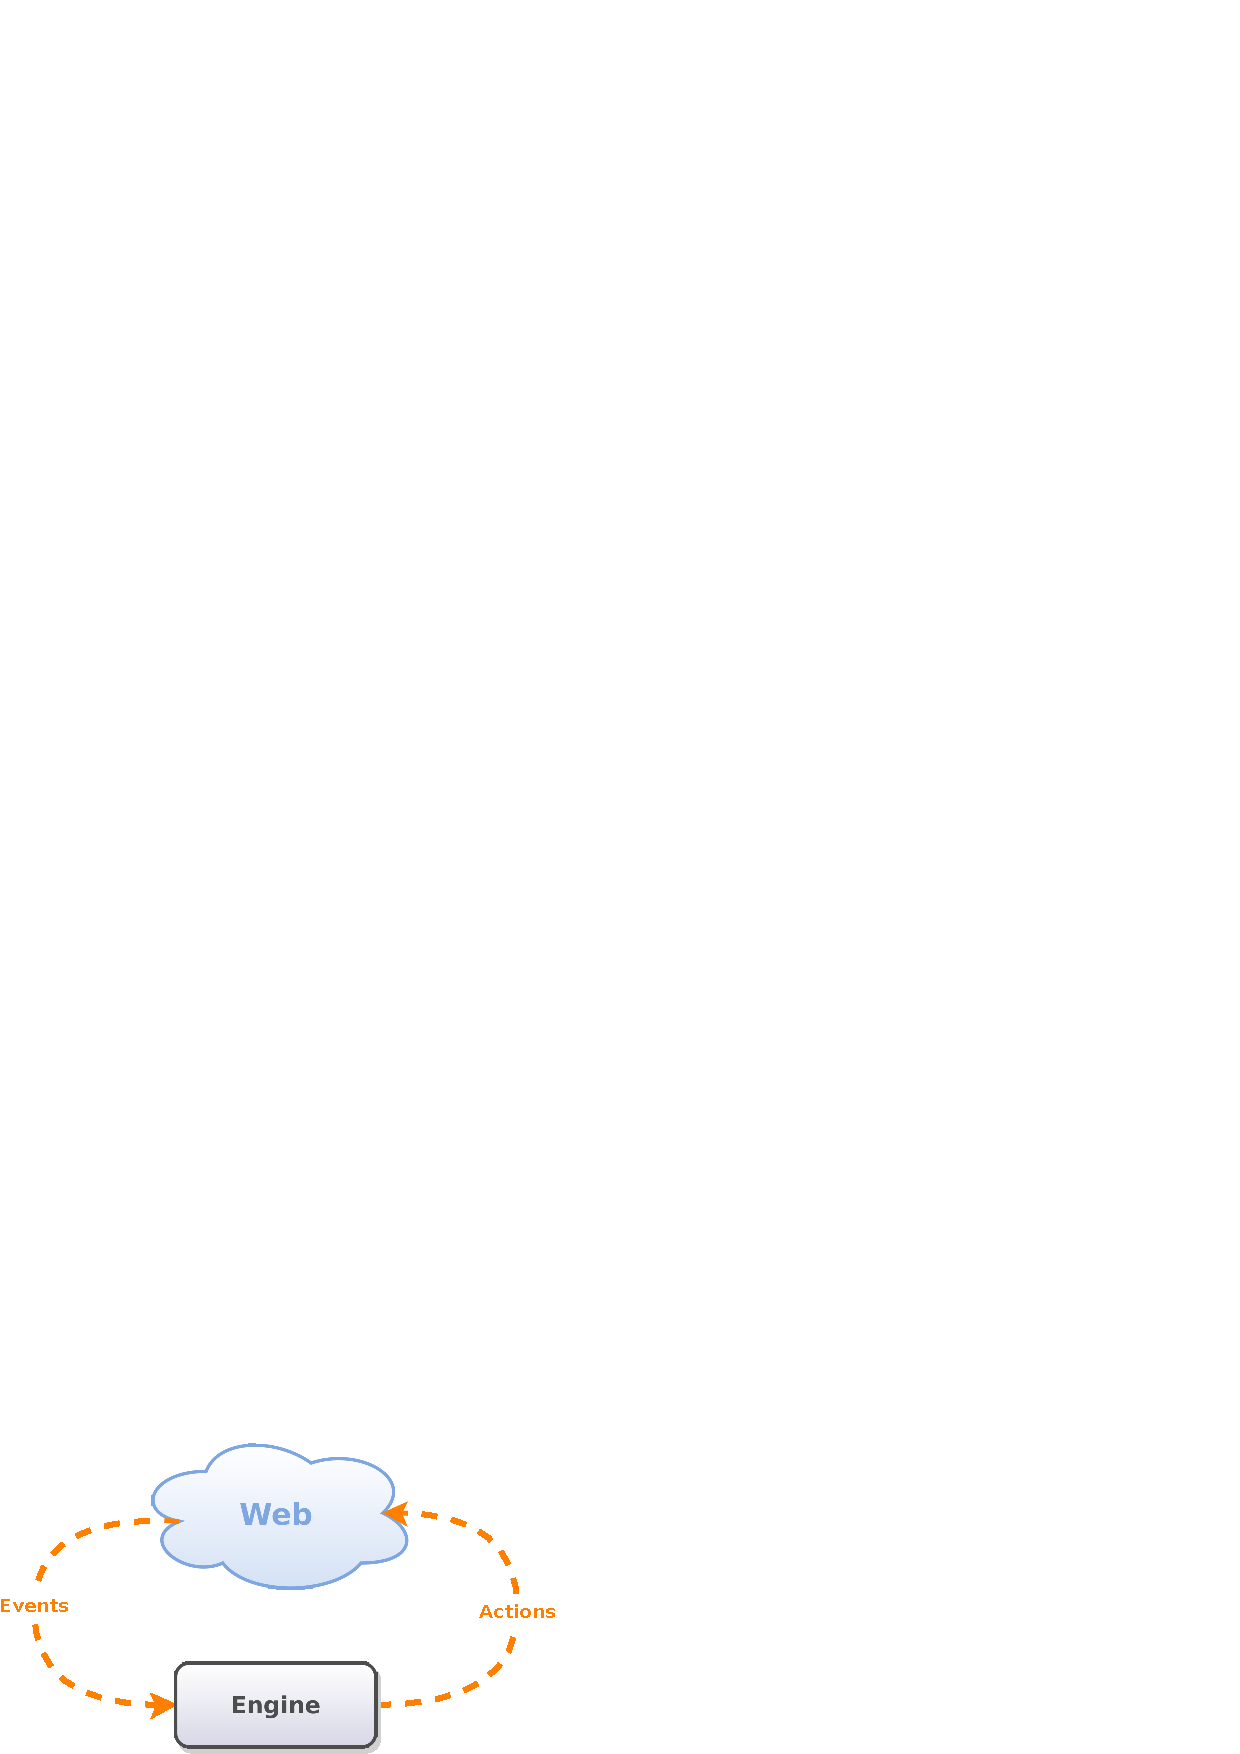
\includegraphics{figures/Conceptual_Model_Simple}
  \caption{Reactor ;) Conceptual model for reactive web systems}
  \label{fig:Conceptual_Model_Simple}
\end{figure}

\begin{figure}[h!]
  \centering
  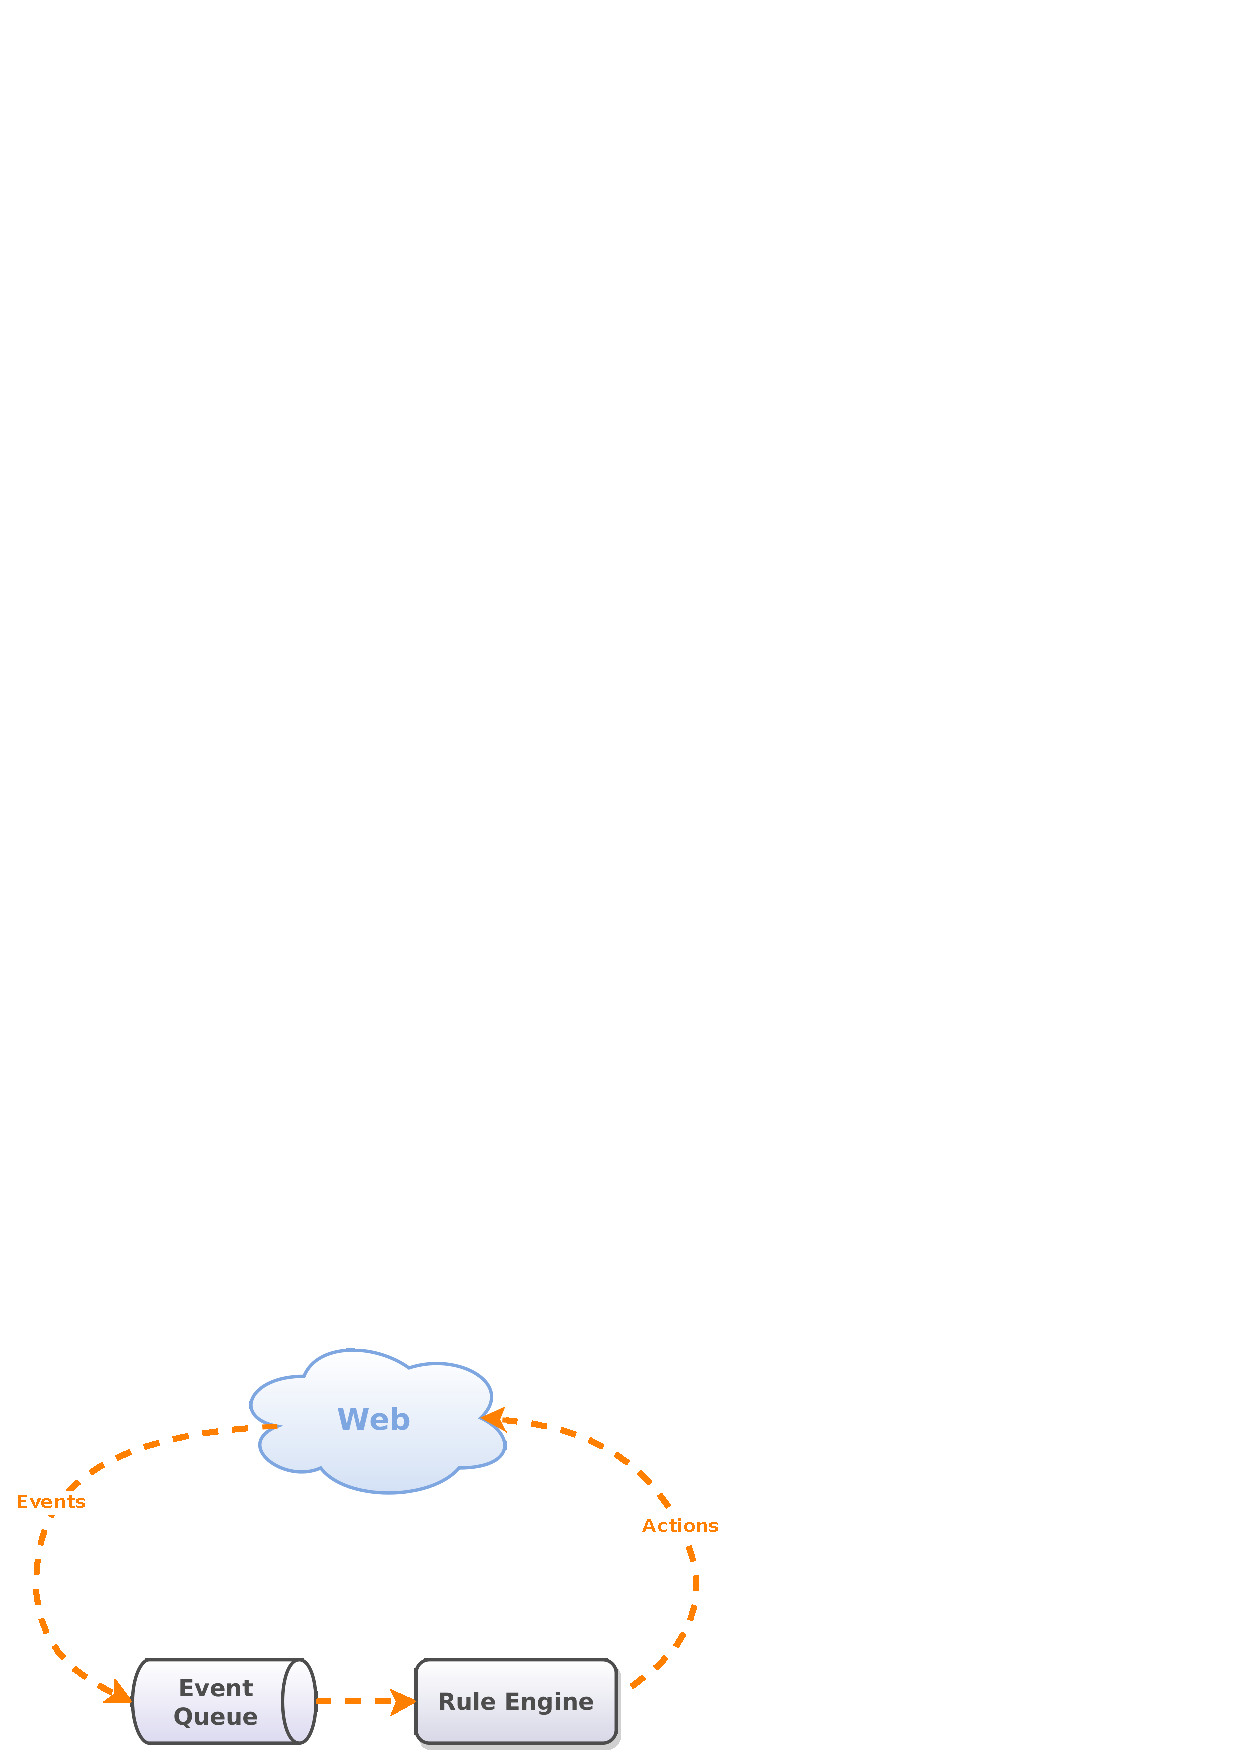
\includegraphics{figures/Conceptual_Model}
  \caption{Conceptual model for reactive Web Systems}
  \label{fig:Conceptual_Model}
\end{figure}


\newpage

\subsubsection{Own Rules}
\begin{Verbatim}[fontsize=\small,commandchars=\\\{\}]
\PY{k}{on} \PY{n}{mail}
\PY{k}{if} \PY{n}{sender}\PY{o}{=}\PY{l+s+ss}{\PYZdq{}sender@mail.com\PYZdq{}}
\PY{k}{do} \PY{n}{webapi}\PY{o}{\PYZhy{}}\PY{o}{\PYZgt{}}\PY{l+s+s2}{newcontent}\PY{p}{(}\PY{n}{subject}\PY{p}{)}
\end{Verbatim}

Would be translated into:

\begin{Verbatim}[fontsize=\small,commandchars=\\\{\}]
\PY{p}{\PYZob{}}
  \PY{n+nt}{\PYZdq{}event\PYZdq{}}\PY{p}{:} \PY{l+s+s2}{\PYZdq{}mail\PYZdq{}}\PY{p}{,}
  \PY{n+nt}{\PYZdq{}conditions\PYZdq{}}\PY{p}{:} \PY{p}{[}
    \PY{p}{\PYZob{}} \PY{n+nt}{\PYZdq{}sender\PYZdq{}}\PY{p}{:} \PY{l+s+s2}{\PYZdq{}sender@mail.com\PYZdq{} }\PY{p}{\PYZcb{}}\PY{p}{,}
  \PY{p}{]}\PY{p}{,}
  \PY{n+nt}{\PYZdq{}actions\PYZdq{}}\PY{p}{:} \PY{p}{[}
    \PY{p}{\PYZob{}}
      \PY{n+nt}{\PYZdq{}api\PYZdq{}}\PY{p}{:} \PY{l+s+s2}{\PYZdq{}webapi\PYZdq{}}\PY{p}{,}
      \PY{n+nt}{\PYZdq{}method\PYZdq{}}\PY{p}{:} \PY{l+s+s2}{\PYZdq{}newcontent\PYZdq{}}\PY{p}{,}
      \PY{n+nt}{\PYZdq{}arguments\PYZdq{}}\PY{p}{:} \PY{p}{\PYZob{}}
        \PY{n+nt}{\PYZdq{}text\PYZdq{}}\PY{p}{:} \PY{l+s+s2}{\PYZdq{}\PYZdl{}X.subject\PYZdq{}}
      \PY{p}{\PYZcb{}}
    \PY{p}{\PYZcb{}}
  \PY{p}{]}
\PY{p}{\PYZcb{}}
\end{Verbatim}

\begin{Verbatim}[commandchars=\\\{\}]
\PY{n+nt}{on} \PY{n}{weather}\PY{o}{\PYZhy{}}\PY{o}{\PYZgt{}}\PY{l+s+s2}{tempRaisesAbove}\PY{p}{(}\PY{l+m+mi}{20}\PY{p}{)}
\PY{n+nt}{do} \PY{n}{probinder}\PY{o}{\PYZhy{}}\PY{o}{\PYZgt{}}\PY{l+s+s2}{addContent}\PY{p}{(}\PY{n}{temp}\PY{p}{)}
\end{Verbatim}

\begin{Verbatim}[commandchars=\\\{\}]
\PY{n+nt}{on} \PY{n}{emailyak}\PY{o}{\PYZhy{}}\PY{o}{\PYZgt{}}\PY{l+s+s2}{newMail}
\PY{n+nt}{if} \PY{n}{FromAddress}\PY{o}{=}\PY{l+s+ss}{\PYZdq{}}\PY{l+s+ss}{dominic.bosch.db@gmail.com}\PY{l+s+ss}{\PYZdq{}}
\PY{n+nt}{do} \PY{n}{probinder}\PY{o}{\PYZhy{}}\PY{o}{\PYZgt{}}\PY{l+s+s2}{newContent}\PY{p}{(}\PY{n}{TextBody}\PY{p}{)}
\end{Verbatim}

\begin{Verbatim}[commandchars=\\\{\}]
\PY{n+nt}{on} \PY{n}{probinder}\PY{o}{\PYZhy{}}\PY{o}{\PYZgt{}}\PY{l+s+s2}{unreadContent}
\PY{n+nt}{if} \PY{n}{serviceId}\PY{o}{=}\PY{l+m+mi}{32}
\PY{n+nt}{do} \PY{n}{probinder}\PY{o}{\PYZhy{}}\PY{o}{\PYZgt{}}\PY{l+s+s2}{markread}\PY{p}{(}\PY{n}{id}\PY{p}{)}\PY{p}{,}
   \PY{n}{probinder}\PY{o}{\PYZhy{}}\PY{o}{\PYZgt{}}\PY{l+s+s2}{createContent}\PY{p}{(}\PY{n}{id}\PY{p}{,} \PY{n}{title}\PY{p}{,} \PY{n}{tab_name}\PY{p}{)}
\end{Verbatim}

\newpage

\begin{Verbatim}[commandchars=\\\{\}]
\PY{k+kd}{function} \PY{n+nx}{call}\PY{p}{(}\PY{n+nx}{args}\PY{p}{)} \PY{p}{\PYZob{}}
  \PY{n+nx}{require}\PY{p}{(}\PY{l+s+s1}{\PYZsq{}needle\PYZsq{}}\PY{p}{)}\PY{p}{.}\PY{n+nx}{post}\PY{p}{(}
    \PY{l+s+s1}{\PYZsq{}https://probinder.com/service/\PYZsq{}} 
      \PY{o}{+} \PY{n+nx}{args}\PY{p}{.}\PY{n+nx}{service} \PY{o}{+} \PY{l+s+s1}{\PYZsq{}/\PYZsq{}} \PY{o}{+} \PY{n+nx}{args}\PY{p}{.}\PY{n+nx}{method}\PY{p}{,}
    \PY{n+nx}{args}\PY{p}{.}\PY{n+nx}{data}\PY{p}{,}
    \PY{n+nx}{args}\PY{p}{.}\PY{n+nx}{credentials}
  \PY{p}{)}\PY{p}{;}
\PY{p}{\PYZcb{}}\PY{p}{;}
\end{Verbatim}


\begin{Verbatim}[commandchars=\\\{\}]
\PY{k+kd}{function} \PY{n+nx}{newContent}\PY{p}{(}\PY{n+nx}{txt}\PY{p}{)}\PY{p}{\PYZob{}}
  \PY{n+nx}{call}\PY{p}{(}\PY{p}{\PYZob{}}
    \PY{n+nx}{service}\PY{o}{:} \PY{l+s+s1}{\PYZsq{}27\PYZsq{}}\PY{p}{,}
    \PY{n+nx}{method}\PY{o}{:} \PY{l+s+s1}{\PYZsq{}save\PYZsq{}}\PY{p}{,}
    \PY{n+nx}{data}\PY{o}{:} \PY{p}{\PYZob{}}
      \PY{n+nx}{companyId}\PY{o}{:} \PY{l+s+s1}{\PYZsq{}961\PYZsq{}}\PY{p}{,}
      \PY{n+nx}{context}\PY{o}{:} \PY{l+s+s1}{\PYZsq{}17930\PYZsq{}}\PY{p}{,}
      \PY{n+nx}{text}\PY{o}{:} \PY{n+nx}{txt}
    \PY{p}{\PYZcb{}}
  \PY{p}{\PYZcb{}}\PY{p}{)}\PY{p}{;}
\PY{p}{\PYZcb{}}
\end{Verbatim}

\begin{Verbatim}[commandchars=\\\{\}]
\PY{k}{on} \PY{n}{mail}
\PY{k}{do} \PY{n}{probinder}\PY{o}{\PYZhy{}}\PY{o}{\PYZgt{}}\PY{l+s+s2}{createContent}\PY{p}{(}\PY{n}{subject}\PY{p}{)}
\end{Verbatim}


\begin{Verbatim}[commandchars=\\\{\}]
\PY{k}{on} \PY{n}{mail}
\PY{k}{do} \PY{n}{probinder}\PY{o}{\PYZhy{}}\PY{o}{\PYZgt{}}\PY{l+s+s2}{call}\PY{p}{(}\PY{l+s+ss}{\PYZdq{}27\PYZdq{}}\PY{p}{,}\PY{l+s+ss}{\PYZdq{}save\PYZdq{}}\PY{p}{,}
     \PY{p}{[}\PY{l+s+ss}{\PYZdq{}961\PYZdq{}}\PY{p}{,} \PY{l+s+ss}{\PYZdq{}17930\PYZdq{}}\PY{p}{,} \PY{n}{subject}\PY{p}{]}
   \PY{p}{)}
\end{Verbatim}


\begin{Verbatim}[commandchars=\\\{\}]
\PY{k}{on} \PY{n}{probinder}\PY{o}{\PYZhy{}}\PY{o}{\PYZgt{}}\PY{l+s+s2}{unread}
\PY{k}{if} \PY{n}{serviceId}\PY{o}{=}\PY{l+m+mi}{32}
\PY{k}{do} \PY{n}{probinder}\PY{o}{\PYZhy{}}\PY{o}{\PYZgt{}}\PY{l+s+s2}{setRead}\PY{p}{(}\PY{p}{id}\PY{p}{)}\PY{p}{,}
   \PY{n}{probinder}\PY{o}{\PYZhy{}}\PY{o}{\PYZgt{}}\PY{l+s+s2}{makeFileEntry}\PY{p}{(}\PY{n}{service}\PY{p}{,} \PY{p}{id}\PY{p}{)}
\end{Verbatim}

\newpage


\begin{Verbatim}[commandchars=\\\{\}]
    \PY{n+nt}{\PYZdq{}event\PYZdq{}}\PY{err}{:} \PY{l+s+s2}{\PYZdq{}emailyak\PYZhy{}\PYZgt{}newMail\PYZdq{}}\PY{err}{,}
    \PY{n+nt}{\PYZdq{}condition\PYZdq{}}\PY{err}{:} \PY{p}{\PYZob{}} \PY{n+nt}{\PYZdq{}FromAddress\PYZdq{}}\PY{p}{:} \PY{l+s+s2}{\PYZdq{}dominic.bosch.db@gmail.com\PYZdq{}}\PY{p}{\PYZcb{}}\PY{err}{,}
    \PY{n+nt}{\PYZdq{}actions\PYZdq{}}\PY{err}{:} \PY{p}{[}
      \PY{p}{\PYZob{}}
        \PY{n+nt}{\PYZdq{}module\PYZdq{}}\PY{p}{:} \PY{l+s+s2}{\PYZdq{}probinder\PYZhy{}\PYZgt{}newContent\PYZdq{}}\PY{p}{,}
        \PY{n+nt}{\PYZdq{}arguments\PYZdq{}}\PY{p}{:} \PY{p}{\PYZob{}}
          \PY{n+nt}{\PYZdq{}content\PYZdq{}}\PY{p}{:} \PY{l+s+s2}{\PYZdq{}Received from EmailYak: \PYZdl{}X.TextBody\PYZdq{}}
        \PY{p}{\PYZcb{}}
      \PY{p}{\PYZcb{}}
    \PY{p}{]}
\end{Verbatim}

\begin{Verbatim}[commandchars=\\\{\}]
\PY{k+kd}{function} \PY{n+nx}{newMail}\PY{p}{(}\PY{n+nx}{callback}\PY{p}{)} \PY{p}{\PYZob{}}
  \PY{n+nx}{needle}\PY{p}{.}\PY{n+nx}{get}\PY{p}{(}\PY{l+s+s1}{\PYZsq{}https://api.emailyak.com/v1/\PYZsq{}}\PY{o}{+}\PY{n+nx}{key}\PY{o}{+}\PY{l+s+s1}{\PYZsq{}/json/get/new/email/\PYZsq{}}\PY{p}{,}
    \PY{k+kd}{function} \PY{p}{(}\PY{n+nx}{error}\PY{p}{,} \PY{n+nx}{response}\PY{p}{,} \PY{n+nx}{body}\PY{p}{)}\PY{p}{\PYZob{}}
        \PY{k+kd}{var} \PY{n+nx}{mails} \PY{o}{=} \PY{n+nx}{JSON}\PY{p}{.}\PY{n+nx}{parse}\PY{p}{(}\PY{n+nx}{body}\PY{p}{)}\PY{p}{.}\PY{n+nx}{Emails}\PY{p}{;}
        \PY{k}{for}\PY{p}{(}\PY{k+kd}{var} \PY{n+nx}{i} \PY{o}{=} \PY{l+m+mi}{0}\PY{p}{;} \PY{n+nx}{i} \PY{o}{\PYZlt{}} \PY{n+nx}{mails}\PY{p}{.}\PY{n+nx}{length}\PY{p}{;} \PY{n+nx}{i}\PY{o}{++}\PY{p}{)} \PY{n+nx}{callback}\PY{p}{(}\PY{n+nx}{mails}\PY{p}{[}\PY{n+nx}{i}\PY{p}{]}\PY{p}{)}\PY{p}{;}
    \PY{p}{\PYZcb{}}
  \PY{p}{)}\PY{p}{;}
\PY{p}{\PYZcb{}}
\end{Verbatim}

\begin{Verbatim}[commandchars=\\\{\}]
\PY{p}{\PYZob{}}
  
  \PY{n+nt}{\PYZdq{}event\PYZdq{}}\PY{p}{:} \PY{l+s+s2}{\PYZdq{}emailyak\PYZhy{}\PYZgt{}newMail\PYZdq{}}\PY{p}{,}
  \PY{n+nt}{\PYZdq{}ToAddressList\PYZdq{}}\PY{p}{:} \PY{l+s+s2}{\PYZdq{}test@mscliveweb.simpleyak.com\PYZdq{}}\PY{p}{,}
  \PY{n+nt}{\PYZdq{}FromAddress\PYZdq{}}\PY{p}{:} \PY{l+s+s2}{\PYZdq{}dominic.bosch.db@gmail.com\PYZdq{}}\PY{p}{,}
  \PY{n+nt}{\PYZdq{}TextBody\PYZdq{}}\PY{p}{:} \PY{l+s+s2}{\PYZdq{}Lengthy body [...]\PYZdq{}}\PY{p}{,}
  \PY{n+nt}{\PYZdq{}Subject\PYZdq{}}\PY{p}{:} \PY{l+s+s2}{\PYZdq{}Fwd: test subject\PYZdq{}}\PY{p}{,}
  \PY{err}{[}\PY{err}{.}\PY{err}{.}\PY{err}{.}\PY{err}{]}

\PY{p}{\PYZcb{}}
\end{Verbatim}

	
\chapter{The "XYZ" Prototype System}

% NOTES / TODOs:
%
% Architecture scheme, implementation
% callback functions, hot plugin
% js-select selectors
% List of condition operators
% Why JS, why wasnt it used before? is it used now?
% Transactions in businesses, find use case. how would we lose events?
% Terminierungsproblem (compiler bau), loesungsansaetze



\section{Event Triggers}

Event Gathering is the E in ECA and without one of these letters such a system would not run.
It is of utmost importance to find as much as possible ways to get data into a system.



\subsection{Polling for Events}



\subsection{Webhooks}
Which 



\section{Actions}



\section{ECA Rules}



\section{Architecture}



\section{Asynchronous Systems \& Closures}
% NOTES / TODOs:
%
% Variable bindings
% Closures (https://developer.mozilla.org/en-US/docs/Web/JavaScript/Guide/Closures)$
% Closures are functions that refer to independent (free) variables. 
% In other words, the function defined in the closure 'remembers' the environment in which it was created in.

% write about arallel as well?

Certain optimization approaches and programming language concepts require special attention to avoid common pitfalls.
If such approaches and concepts come together, which is the case when closures are used in asynchronous systems, random inconsistencies will be the result if they are not taken care of.


Looking at an example of sequential code execution ( Figure~\ref{fig:Closures_Synchronous} ), we see that function execution of fA is halted until function fB is finished.
If fB happens to be a latency-driven I/O operation the completion of fA could be deferred for a relatively long time.
While the application waits for the completion of the I/O operation, some remaining operations in fA could eventually already be executed without causing any race conditions.

\begin{figure}[h!]
\centering
  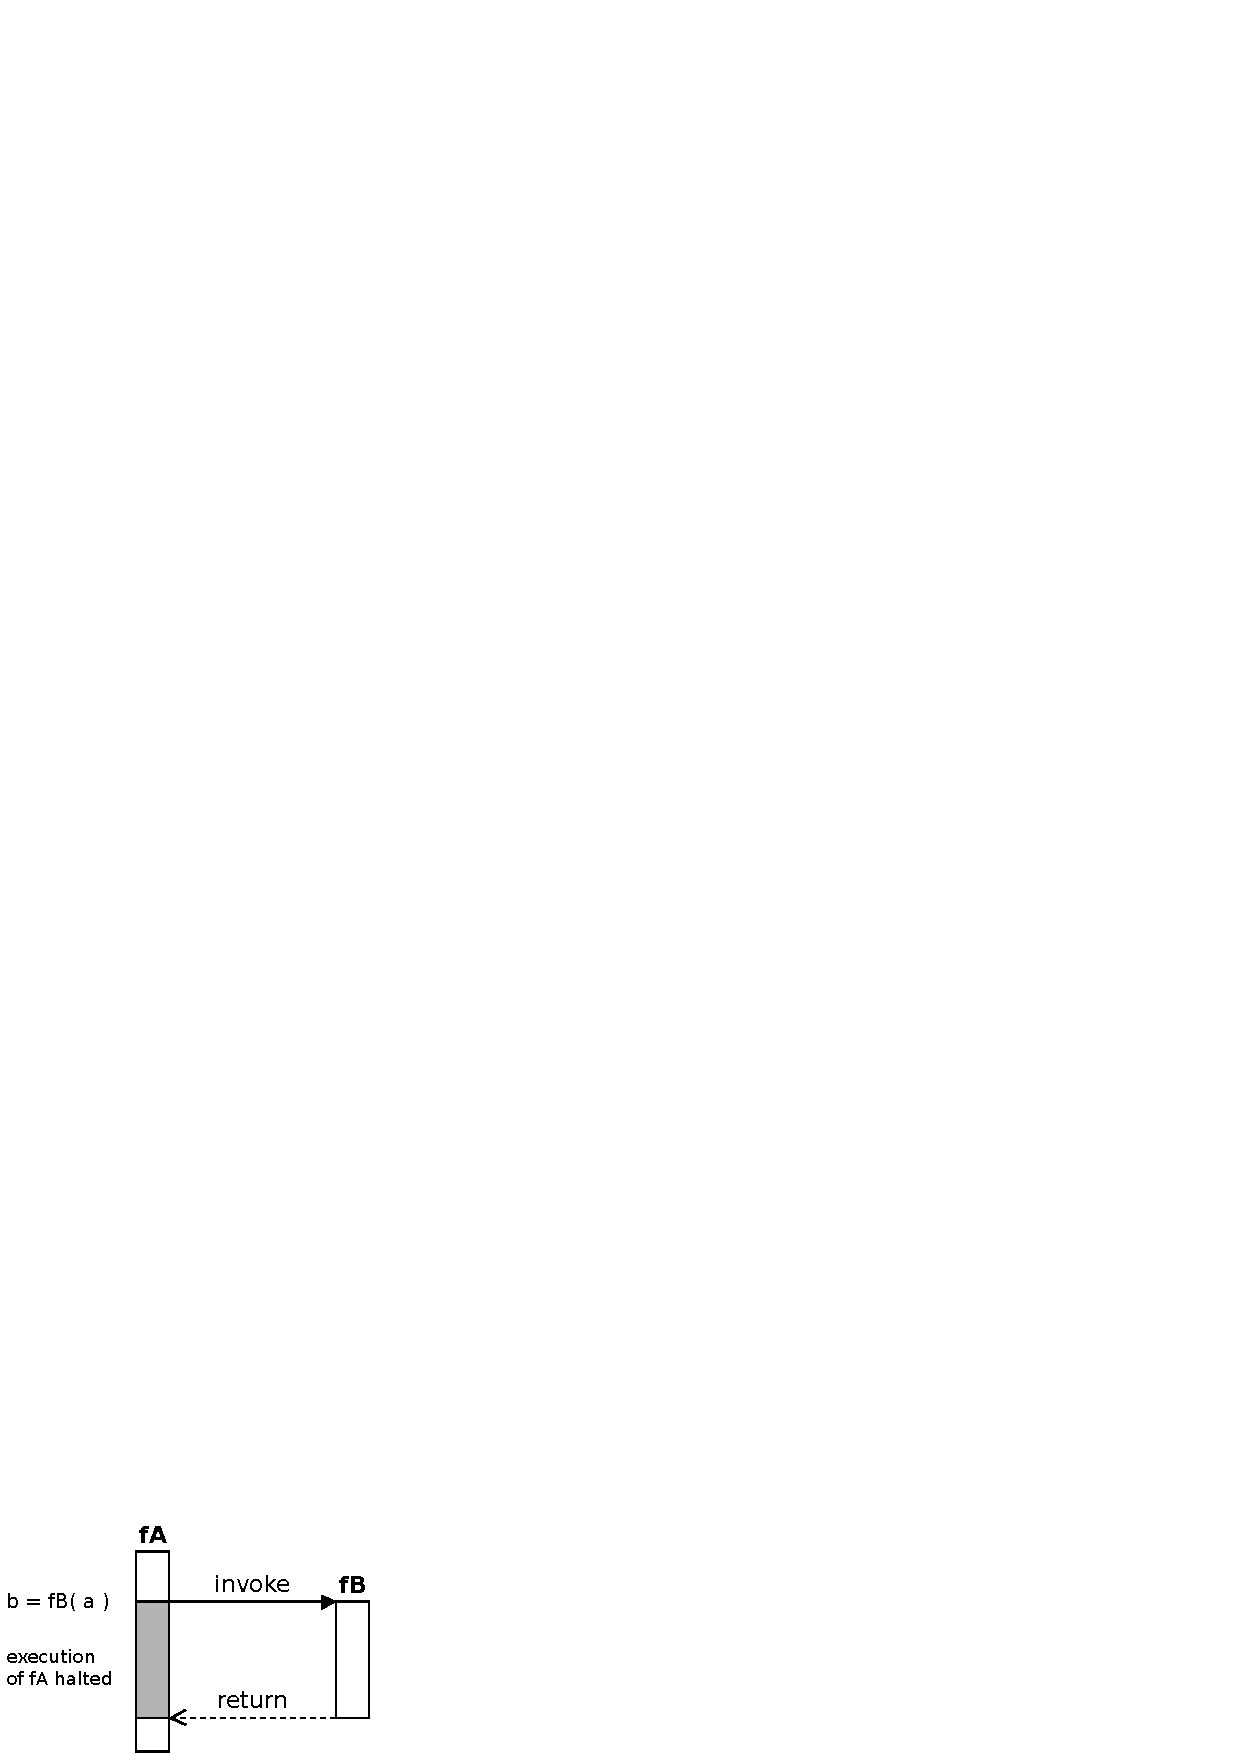
\includegraphics{figures/Closures_Synchronous}
\caption{Synchronous Function Calls}
\label{fig:Closures_Synchronous}
\end{figure}

Non-blocking operations are a remedy for optimzed resource allocation and opens ways to overcome such unnecessary resource bindings.
Asynchronous code execution allows non-blocking and thus scalable applications.
Processing any kind of latency-driven I/O operation asynchronously ( e.g. filesystem access and socket communication ) exploits resources that would otherwise be bound while waiting for completion.
Such operations are processed and completed whenever required resources are available.
Often other operations depend on the completion of asynchronous operations, hence their execution needs to be deferred.
This required code execution deferral is achieved through the application of callback functions.
Any code placed in a callback function, which is assigned to an asynchronous operation, is only executed when the respective asynchronous operation completed.
This leads to stacking of functions and operations



Such callback functions are passed as arguments to asynchronous operations and executed as soon as the operation finishes.

By deferring the executiong of operations that depend on the 

asynchronously results in dynamic code which exploits .

together with closures they 

Test reference Figure ~\ref{fig:Closures_Synchronous}



\begin{figure*}[htb]
%\begin{center}
\centering
%,angle=-90
  \makebox[\textwidth][c]{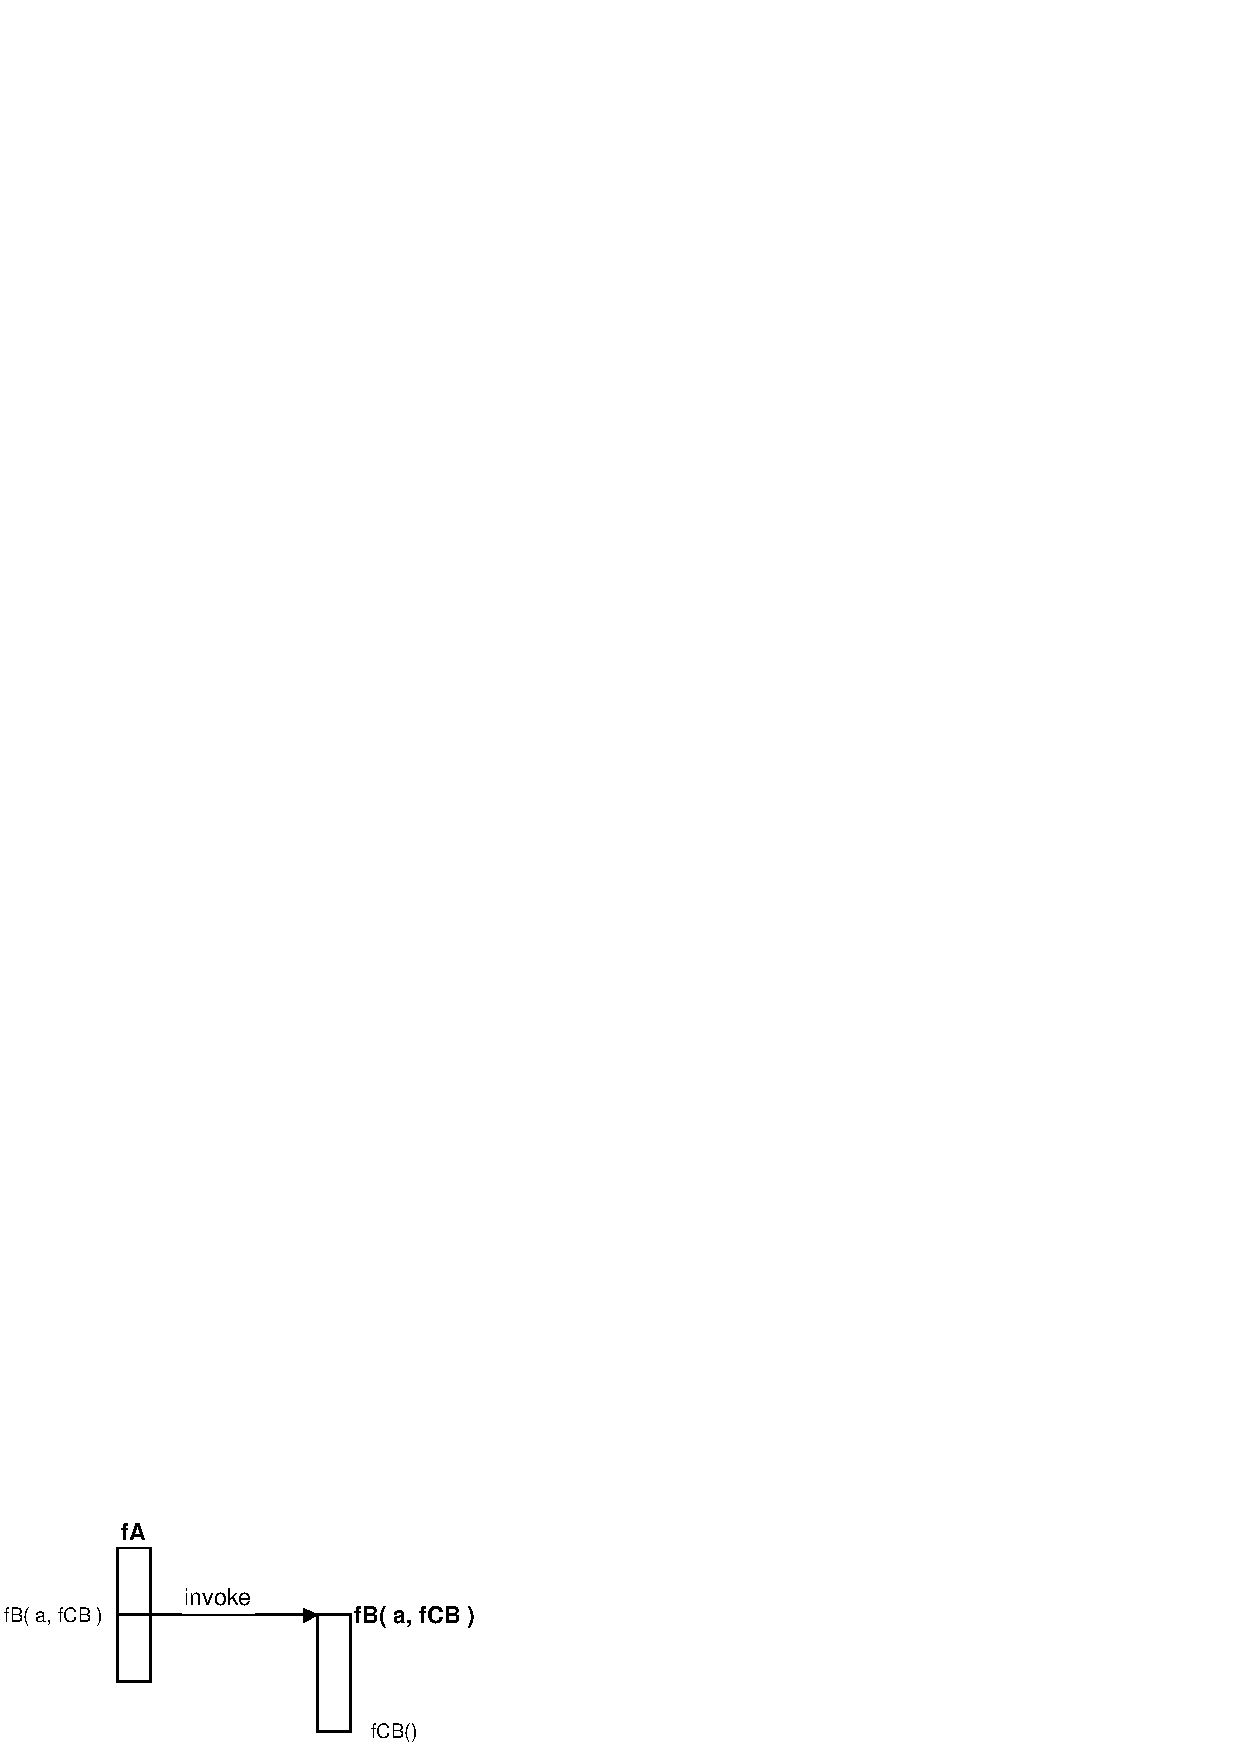
\includegraphics{figures/Closures_Asynchronous}}%
\caption{Asynchronous Function Calls}
%\end{center}
\end{figure*}


\begin{figure*}[htb]
%\begin{center}
\centering
%,angle=-90
  \makebox[\textwidth][c]{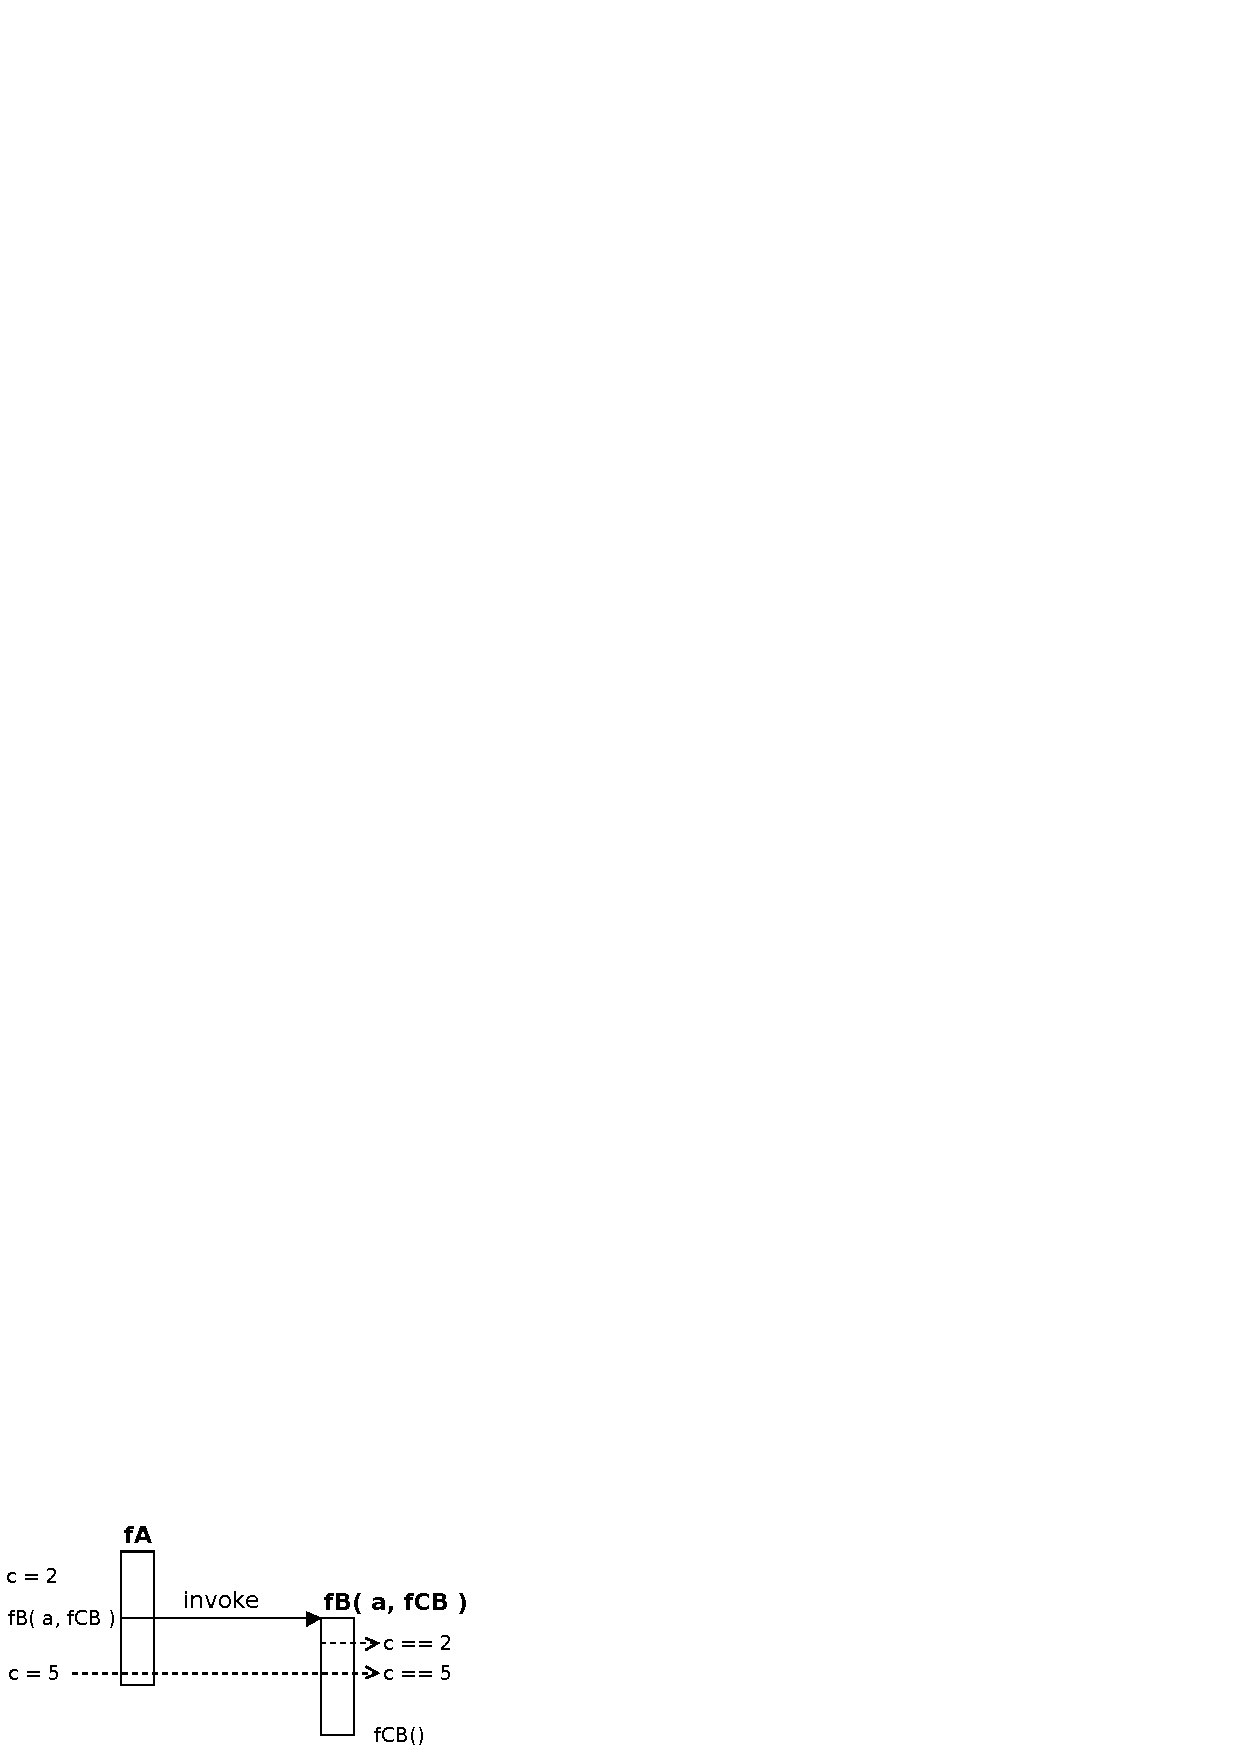
\includegraphics{figures/Closures_Closure-1}}%
\caption{Closure Scope}
%\end{center}
\end{figure*}


\begin{figure*}[htb]
%\begin{center}
\centering
%,angle=-90
  \makebox[\textwidth][c]{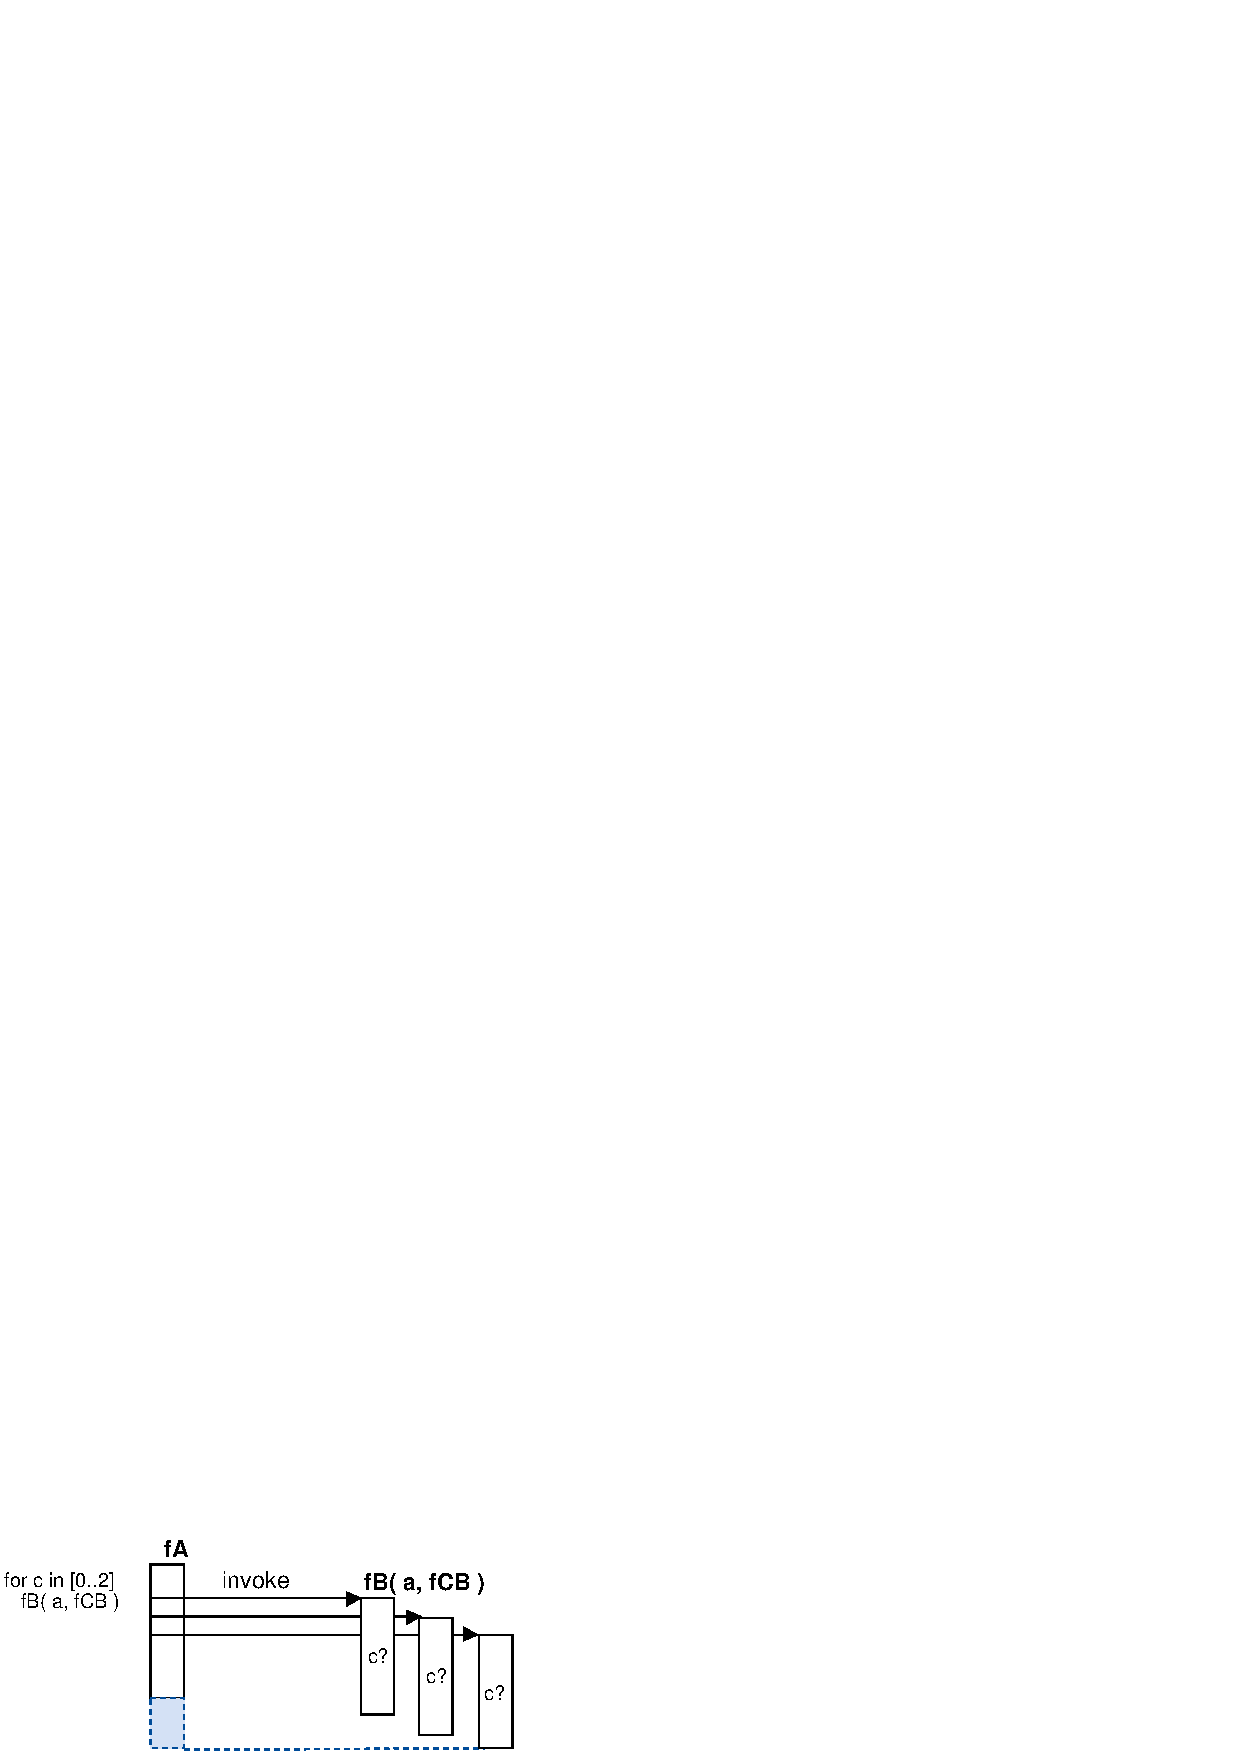
\includegraphics{figures/Closures_Closure-2}}%
\caption{Closure Scope}
%\end{center}
\end{figure*}


\begin{figure*}[htb]
%\begin{center}
\centering
%,angle=-90
  \makebox[\textwidth][c]{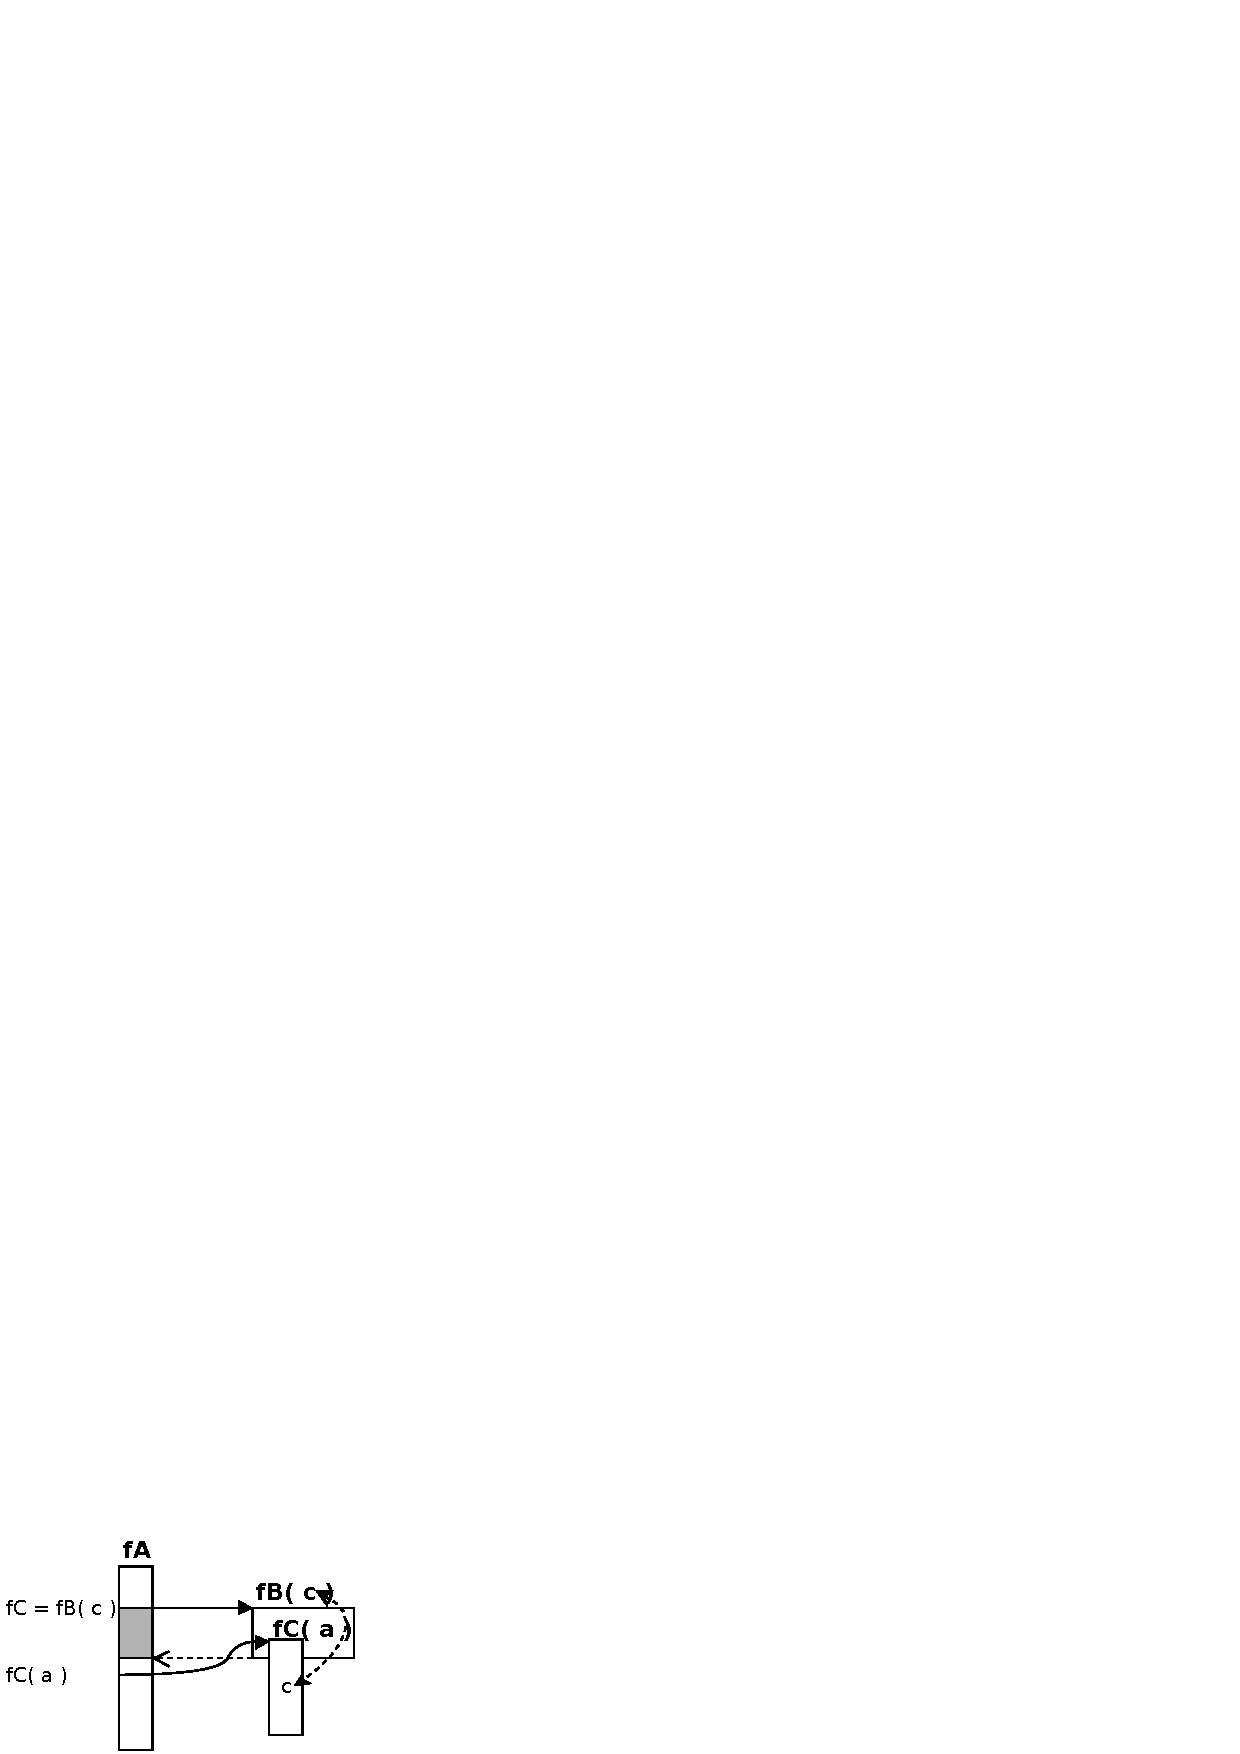
\includegraphics{figures/Closures_Closure-3}}%
\caption{Closure Scope}
%\end{center}
\end{figure*}

% Error tracing
% Apply variable number of function arguments to function

	
\chapter{Discussion \& Results}



% \section{Use Cases}
% NOTES / TODOs:
%
% Temperature warning, using import.io
% Tutorial example: as seen by user, as seen by the developer
%http://khanlou.com/2014/03/model-view-whatever/
% Transactions in businesses, find use case. how would we lose events?


% We are taking a step further and allow not only the chaining up of several remote ECA engines, but also the invocation of actions on any arbitrary Web accessible service.


\section{Use Cases?}


\section{Future Work?}
% NOTES / TODOs:
%
% CEP
We have seen that the ECA approach is already a powerful one to make the web reactive.
A future improvement of this could be to adopt Complex Event Processing (CEP).
This would mean that several events could be stored in a rule and be evaluated in terms of time constraints.
Through this more complex events can be created as a result of several atomic events which would lead into semantically more complex events.
A change in paradigm will result in an approach where events are not just processed when they are entering the system and evaluated against rules, but these events would need to be stored for quite a long time.
Also the rules will not all be checked for each event but they are subject to a scheduler.
It can be decided when and how often a rule is evaluated and all events will be checked at these point in times, whether they are candidates for firing the rule.
A relational database will be needed in order to search through the timestamps

% Transactions for business. find use case.and explain how we would loose events.
% TODO pathologische beispiele
% Endless loops -> child_process to be killed when not responding. what about async callbacks?


\backmatter
	
\renewcommand*\appendixtocname{Appendix}
\begin{appendices}
\addtocontents{toc}{\protect\setcounter{tocdepth}{-1}}
\chapter{Rules}
\section{Wow}
\subsection{Binder voila}
% \begin{Verbatim}[fontsize=\small,commandchars=\\\{\}]
% \PY{l+s}{\PYZsq{}}\PY{l+s}{use strict}\PY{l+s}{\PYZsq{}}\PY{p}{;}
% \PY{n}{var} \PY{n}{express} \PY{o}{=} \PY{n}{require}\PY{p}{(}\PY{l+s}{\PYZsq{}}\PY{l+s}{express}\PY{l+s}{\PYZsq{}}\PY{p}{)}\PY{p}{;}
% \PY{n}{var} \PY{n}{qs} \PY{o}{=} \PY{n}{require}\PY{p}{(}\PY{l+s}{\PYZsq{}}\PY{l+s}{querystring}\PY{l+s}{\PYZsq{}}\PY{p}{)}\PY{p}{;}
% \PY{n}{var} \PY{n}{engine} \PY{o}{=} \PY{n}{require}\PY{p}{(}\PY{l+s}{\PYZsq{}}\PY{l+s}{./ecainference}\PY{l+s}{\PYZsq{}}\PY{p}{)}\PY{p}{;}
% \end{Verbatim}

% \begin{lstlisting}[caption=My Javascript Example]
% Name.prototype = {
%   methodName: function(params){
%     var doubleQuoteString = "some text";
%     var singleQuoteString = 'some more text';
%     // this is a comment
%     if(this.confirmed != null && typeof(this.confirmed) == Boolean && this.confirmed == true){
%       document.createElement('h3');
%       $('#system').append("This looks great");
%       return false;
%     } else {
%       throw new Error;
%     }
%   }
% }
% \end{lstlisting}
 % \section{ECA Rules Engine Resources}
  %  \subsection{Node.js Rules Engine Code}
   % \subsubsection{ecaserver.js}

    \begin{Verbatim}[fontsize=\small,commandchars=\\\{\}]
    \PY{l+s}{\PYZsq{}}\PY{l+s}{use strict}\PY{l+s}{\PYZsq{}}\PY{p}{;}
    \PY{n}{var} \PY{n}{express} \PY{o}{=} \PY{n}{require}\PY{p}{(}\PY{l+s}{\PYZsq{}}\PY{l+s}{express}\PY{l+s}{\PYZsq{}}\PY{p}{)}\PY{p}{;}
    \PY{n}{var} \PY{n}{qs} \PY{o}{=} \PY{n}{require}\PY{p}{(}\PY{l+s}{\PYZsq{}}\PY{l+s}{querystring}\PY{l+s}{\PYZsq{}}\PY{p}{)}\PY{p}{;}
    \PY{n}{var} \PY{n}{engine} \PY{o}{=} \PY{n}{require}\PY{p}{(}\PY{l+s}{\PYZsq{}}\PY{l+s}{./ecainference}\PY{l+s}{\PYZsq{}}\PY{p}{)}\PY{p}{;}
    \end{Verbatim}
%t.b.d.


\chapter{Rules Too}
\section{Wow}
\subsection{Binder voila}
\end{appendices}
\addtocontents{toc}{\protect\setcounter{tocdepth}{0}}
	\addcontentsline{toc}{chapter}{Bibliography}
	\bibliography{thesisbib}
	\bibliographystyle{thesisbst}
	\listoffigures
	\listoftables
	\lstlistoflistings
	\addcontentsline{toc}{chapter}{Index}
	\printindex
\end{document}
